\documentclass[lualatex,book,paper=a4paper,jafontsize=11.5pt,jafontscale=1.05]{jlreq}

% フォント
\usepackage{luatexja-fontspec}
\usepackage{hack-fonts}

% 表紙
\usepackage{hack-cover}

% リンク
\usepackage[hidelinks]{hyperref}

% 画像
\usepackage{graphicx}

% 表
\usepackage{booktabs}
\usepackage{array}
\usepackage{tabularx}
\usepackage{float}
\usepackage{longtable}

% 数式
\usepackage{amsmath}

% コード
\usepackage{listings}
\usepackage{xcolor}

% リスト
\usepackage{enumitem}

\lstset{
  basicstyle=\ttfamily\small,
  frame=single,
  breaklines=true,
  numbers=left,
  numberstyle=\tiny\color{gray},
  keywordstyle=\color{blue}\bfseries,
  commentstyle=\color{green!50!black},
  stringstyle=\color{orange},
  backgroundcolor=\color{gray!8},
  tabsize=2,
}

% 図スペース用コマンド
\newcommand{\figspace}[2][4]{%
  \begin{figure}[H]
    \centering
    \fbox{\begin{minipage}{0.92\linewidth}
      \centering\vspace{#1cm}
      \textit{（#2）}
      \vspace{#1cm}
    \end{minipage}}
  \end{figure}
}

% =============================================================
\title{Arduinoオーケストラ}
\subtitle{〜楽器間同期演奏システム〜}
\team{グループ32}
\author{
  25G1033 : 長見 東磨\\
  25G1098 : 長野 志哉\\
  25G1099 : 長山 魁良\\
  25G1094 : 中村 海惺\\
  \mbox{} : 飛田\\
  \mbox{} : 慶田\\
  \mbox{} : 尾添
}
\date{2026年5月13日}
\version{1.0}

% =============================================================
\begin{document}
\maketitle

\setcounter{tocdepth}{2}
\tableofcontents \thispagestyle{empty}

% =============================================================
\chapter{プロジェクトの計画書}\label{chap:project-plan}\setcounter{page}{1}

% =====================
\section{プロジェクトの概要}

\subsection{プロジェクトの題目}
指揮者人形による自律同期Arduinoオーケストラ

\subsection{プロジェクトの目的}

音楽の自動演奏システムは数多く存在するが，その大半は事前に定義された楽譜とテンポを機械的に再生するに留まり，演奏中の人間的な表現が介在する余地は乏しい．とりわけ，指揮者がリアルタイムに与えるアゴーギク，\textit{accelerando}（加速），\textit{ritardando}（減速），フェルマータ（音の引き伸ばし）といったテンポと時間の揺らぎは，音楽の重要な要素の一つである．Borchersらが Personal Orchestra として実装した研究\cite{borchers2004personal}以降，指揮動作を入力として演奏速度を変更するシステムは複数提案されてきたが，その多くは中央のサーバが指揮を解釈して各音源に同期信号を配信する集中型アーキテクチャを採用しており，人間のオーケストラに見られる「各奏者が指揮者を観測して同期する」という分散的構造とは異なる．

本プロジェクトの目的は，指揮者ロボットの物理的動作を各楽器ユニットが独立に観測し，その指揮表現にリアルタイムに追従して合奏する電子アンサンブルシステムを構築することである．具体的には，サーボモータで反射板を駆動して指揮動作を再現する親機と，赤外線距離センサおよびフォトトランジスタで親機を観測する複数の楽器ユニットからなる構成をとり，ユニット間通信を介さない物理的観測のみで同期演奏を実現する．最終的なゴールは，\textit{accelerando}，\textit{ritardando}，フェルマータといった指揮の表現変化に対し，各楽器ユニットがそれぞれ追従して合奏できる状態を達成することである．

本プロジェクトにおいて解決すべき技術的課題は，以下の二点である．まず，単一のセンサでは拍タイミングの精度と動作変化の連続観測を両立できないため，フォトトランジスタによる発光検出と赤外線センサによる距離測定を統合する設計が必要となる．次に，過去の拍履歴から滑らかなテンポ追従を行いつつ，\textit{accelerando}/\textit{ritardando}による急な変化やフェルマータによる時間の停止を遅滞なく検出する必要がある．

\subsection{既存の技術とプロジェクトの独自性}

\subsubsection{既存の技術}

機械による自動演奏および指揮・演奏への追従に関する研究は，大きく以下の二系統に分類される．

\paragraph{楽譜追従システム}
人間奏者の演奏音響をリアルタイム解析し，楽譜上の現在位置を推定して伴奏を行うシステムである．ContがIRCAMで開発したAntescofo\cite{cont2008antescofo}はその代表例であり，確率的推論によって奏者の演奏位置と速度を追跡しながら，電子音響パートを同期させる．これらのシステムは演奏に対して高度に追従するが，追従対象は奏者の音響であり，指揮者の動作ではない．

\paragraph{指揮認識システム}
カメラやモーションセンサで指揮者の動きを取得し，テンポや音量に変換するシステムである．BorchersらのPersonal Orchestra\cite{borchers2004personal}は赤外線バトンを用いた指揮動作認識により，録音をリアルタイムに伸縮させて再生する．本系統の研究の多くは，中央サーバが指揮を解釈し，その結果を音源へ配信する集中型アーキテクチャを採用する．

\subsubsection{プロジェクトの独自性}

上記の既存研究を踏まえ，本プロジェクトは以下の二点に独自性を持つ．

\paragraph{指揮の表現を物理的に直接観測する設計}
従来の指揮認識システムがカメラ画像や専用バトンの信号を介して指揮を解釈するのに対し，本プロジェクトでは各楽器ユニットが指揮者ロボットを赤外線センサとフォトトランジスタで直接観測する．これにより，振りの速度変化（\textit{accel.}/\textit{rit.}）と最下点での停滞（フェルマータ）という指揮者の表現情報を，加工を経ない一次情報として各楽器が受け取る．

\paragraph{2系統のセンサ統合による拍検出の頑健化}
赤外線距離センサによる連続的な腕位置観測と，フォトトランジスタによる発光検出という二つの独立した観測系を組み合わせる．後者は時間分解能に優れ拍の瞬間を高精度に捉えられる一方，前者は最下点予測やフェルマータ検出といった連続的な動作状態の判定に適している．両者を指数移動平均（Exponential Moving Average; EMA）に基づくテンポ推定器で統合することで，単一センサでは困難な「拍タイミングの精度」と「テンポ変化への追従」の両立を図る．

% =====================
\section{スコープ・マネジメント}\label{sec:scope}

\subsection{成果物}

本プロジェクトで最終的に完成・納品する成果物を以下に示す．

\begin{description}
  \item[ハードウェア]
    \begin{itemize}
      \item 指揮者人形ユニット（サーボ機構・腕・反射板）
      \item 指揮者回路（LED駆動回路・サーボ駆動回路）
      \item フォトトランジスタ配線・遮光チャンバー
    \end{itemize}
  \item[ソフトウェア]
    \begin{itemize}
      \item 指揮者Arduino SW（サーボ制御・カラーLED制御）
      \item 観測Arduino SW（センサーISR・EMAテンポ推定・状態機械）
      \item 演奏Arduino SW $\times$ 5（カラーキュー待受・楽譜進行・シリアル送信）
      \item 楽譜配列データ（「かえるのうた」5パート分）
      \item Processing音響合成SW（シリアル受信・倍音合成・ADSR・エフェクト）
      \item 音色定義データ・ADSRパラメータシート
    \end{itemize}
  \item[ドキュメント]
    \begin{itemize}
      \item マネジメント計画書（本文書）
      \item システム基本設計書（第2章）
      \item システム詳細設計書（第3章）
    \end{itemize}
\end{description}

\subsection{プロジェクトの対象範囲と非対象範囲}

\subsubsection{対象範囲}
本プロジェクトが取り組む範囲を以下に示す．
\begin{itemize}
  \item 指揮者人形ユニットの設計・製作（機構・回路・ソフトウェア）
  \item 赤外線センサおよびフォトトランジスタによる拍タイミング検出
  \item 指数移動平均（EMA）を用いたリアルタイムテンポ推定
  \item 「かえるのうた」5パート輪唱の同期演奏制御
  \item テンポ変化（\textit{accelerando}/\textit{ritardando}）およびフェルマータへのリアルタイム追従
  \item Processingによる音響合成およびスピーカへの出力
\end{itemize}

\subsubsection{非対象範囲}
以下は本プロジェクトの対象外とする．
\begin{itemize}
  \item 「かえるのうた」以外の楽曲への対応
  \item Arduinoユニット間のワイヤレス（無線）通信
  \item 演奏中のリアルタイム楽曲切り替え機能
  \item スマートフォンやWebブラウザからの外部制御インターフェース
  \item 製品化・量産を前提とした耐久性設計
\end{itemize}

\subsection{機能分解構造FBS}

機能分解構造（FBS：Function Breakdown Structure）は，システムが果たすべき機能を階層的に分解したものである．
本プロジェクトのFBSを図\ref{fig:fbs}に示す．

最上位（L0）の「Arduinoオーケストラシステム」を，5つの主機能グループ（L1）に分解する．
\begin{itemize}
  \item \textbf{指揮動作検出}：フォトトランジスタと赤外線センサにより拍タイミングを検出し，EMAでテンポを推定する．フェルマータや見逃し補完も含む．
  \item \textbf{指揮者人形動作}：サーボモータで腕を往復させてテンポを物理提示し，最下点でLEDを点灯させることで拍の同期基準を与える．
  \item \textbf{演奏制御}：親機からのカラーキューによる演奏開始制御，楽譜進行，テンポ追従演奏の3機能を担う．
  \item \textbf{音響合成}：倍音・ADSRによる音色合成，エフェクト付与，フェルマータ時の延奏を行う．
  \item \textbf{状態管理}：待機・予備拍・演奏中・フェルマータ等の状態遷移を管理し，異常時のフォールバックを提供する．
\end{itemize}

\begin{figure}[H]
  \centering
  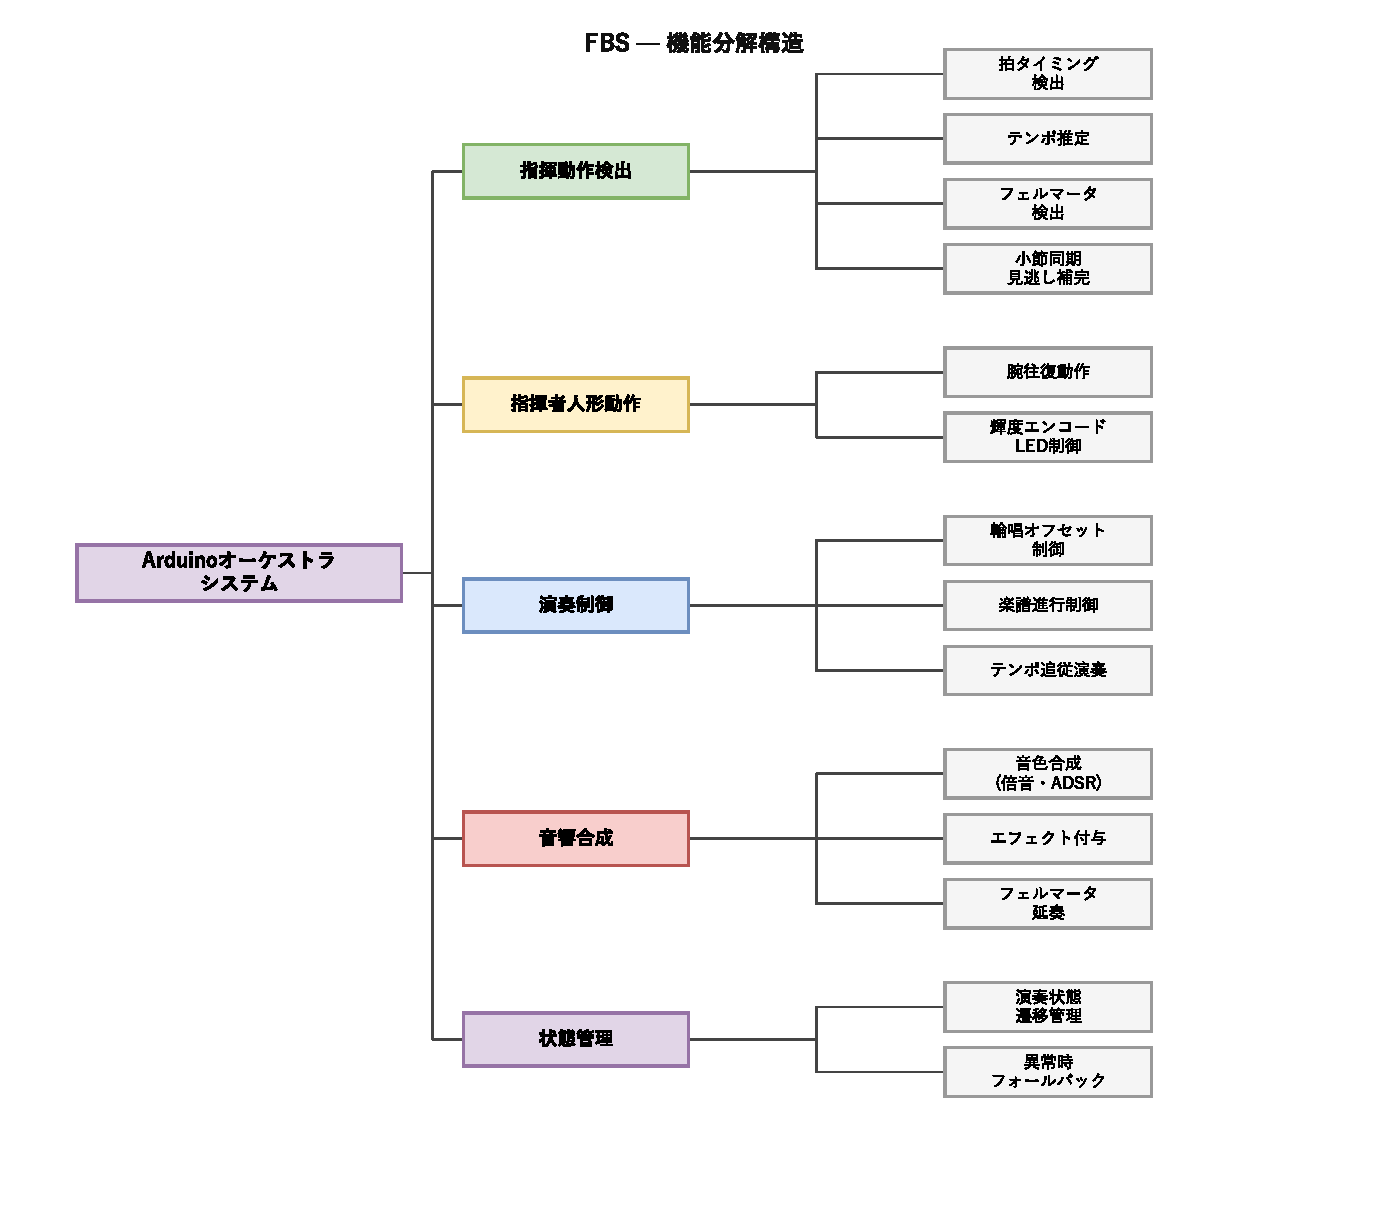
\includegraphics[width=\linewidth]{figures/common/fbs.drawio.pdf}
  \caption{機能分解構造（FBS）}
  \label{fig:fbs}
\end{figure}

\subsection{製品分解構造PBS}

製品分解構造（PBS：Product Breakdown Structure）は，システムを構成する成果物（ハードウェア・ソフトウェア・データ）を階層的に分解したものである．
本プロジェクトのPBSを図\ref{fig:pbs}に示す．

最上位（L0）を担当単位（L1）で分割し，各担当の成果物（L2）およびその構成要素（L3）まで展開する．

\begin{itemize}
  \item \textbf{担当A（指揮者人形ユニット）}：サーボ機構・腕・反射板からなる人形機構，カラーLED・サーボ駆動回路，およびサーボ制御・カラーLED制御ソフトウェア，ならびに楽器指定・BPM入力・演奏制御ボタンを備えたProcessing専用GUIインターフェース．
  \item \textbf{担当B（センサー・観測）}：フォトトランジスタ配線（遮光チャンバー含む），カラーセンサ配線，センサーISR・EMAテンポ推定・状態機械・カラーキュー判別を実装した観測Arduino SW．
  \item \textbf{担当C（演奏制御）}：カラーキュー受信・楽譜進行・シリアル送信を実装した演奏Arduino SW，および「かえるのうた」5パート分の楽譜配列データ．
  \item \textbf{担当D（音響合成）}：シリアル受信・音色合成エンジン・エフェクト処理を実装したProcessing SW，および音色定義シートとADSRパラメータからなる音色定義データ．
\end{itemize}

\begin{figure}[H]
  \centering
  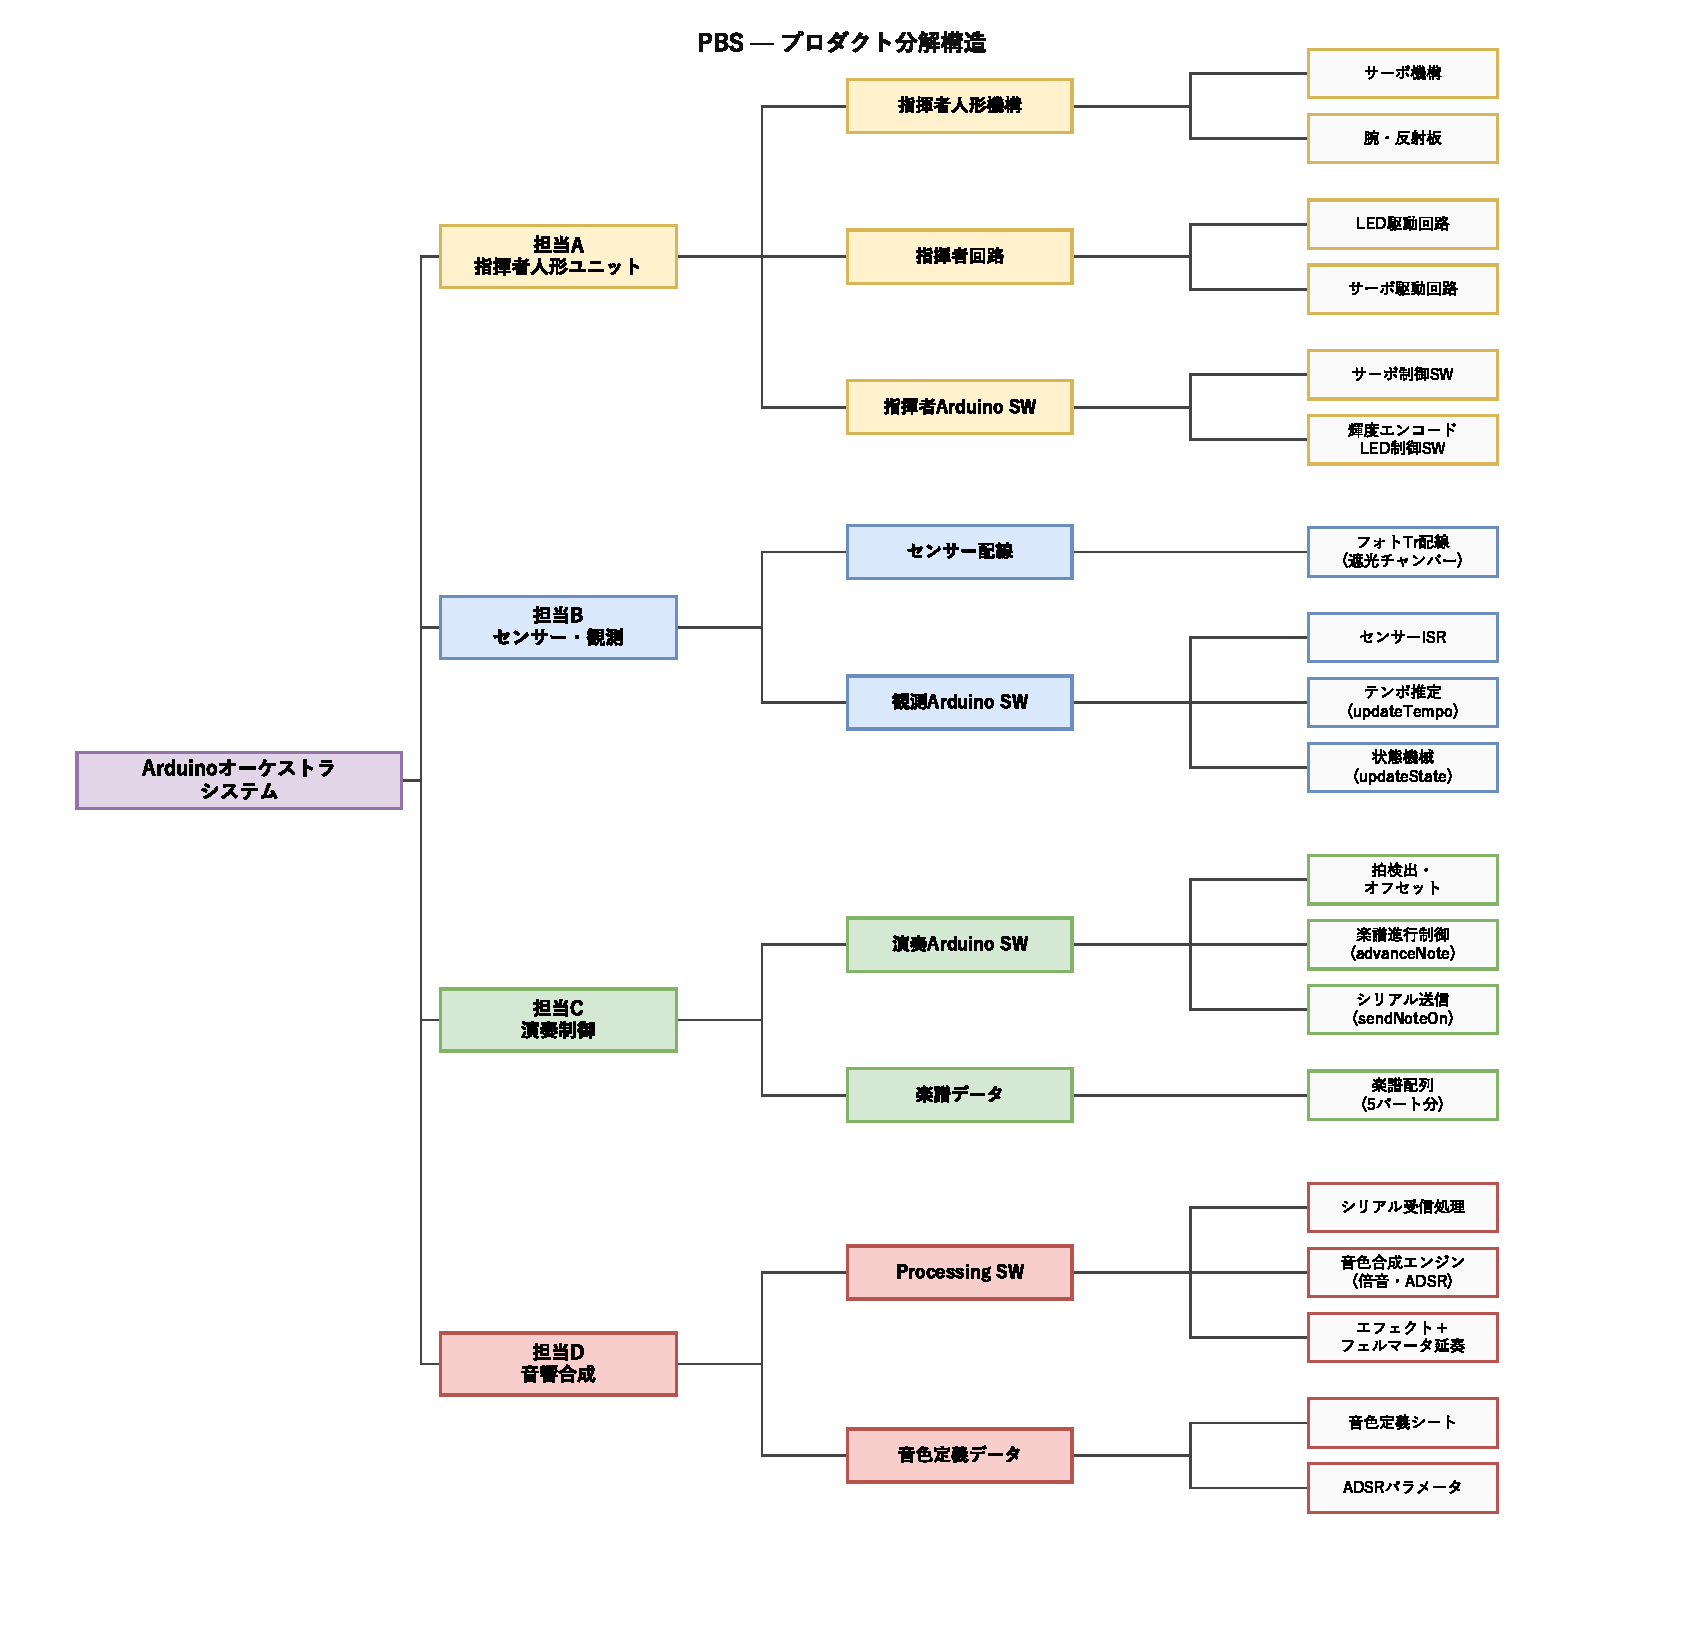
\includegraphics[width=\linewidth]{figures/common/pbs.drawio.pdf}
  \caption{製品分解構造（PBS）}
  \label{fig:pbs}
\end{figure}

\subsection{FBSとPBSの対応関係}

FBSの各機能とPBSの各成果物の対応関係を表\ref{tab:fbs-pbs}に示す．
FBSは「何をするか」，PBSは「何を作るか」を表しており，それぞれの機能は一つ以上の成果物によって実現される．

\begin{table}[H]
  \centering
  \caption{FBS機能とPBS成果物の対応}
  \label{tab:fbs-pbs}
  \begin{tabularx}{\linewidth}{lX}
    \toprule
    FBS機能（L2） & 対応するPBS成果物（L2/L3） \\
    \midrule
    拍タイミング検出    & センサー配線（フォトTr配線），観測Arduino SW（センサーISR） \\
    テンポ推定          & 観測Arduino SW（updateTempo） \\
    フェルマータ検出    & 観測Arduino SW（状態機械） \\
    小節同期・見逃し補完 & 観測Arduino SW（状態機械） \\
    \midrule
    腕往復動作          & 指揮者人形機構（サーボ機構・腕），指揮者回路（サーボ駆動回路），指揮者Arduino SW（サーボ制御SW） \\
    カラーLED制御 & 指揮者回路（カラーLED駆動回路），指揮者Arduino SW（カラーLED制御SW） \\
    \midrule
    演奏開始キュー制御  & カラーセンサ配線，観測Arduino SW（カラーキュー判別・開始フラグ管理） \\
    楽譜進行制御        & 演奏Arduino SW（advanceNote），楽譜データ（楽譜配列） \\
    テンポ追従演奏      & 演奏Arduino SW（sendNoteOn） \\
    \midrule
    音色合成            & Processing SW（音色合成エンジン），音色定義データ（音色定義シート・ADSRパラメータ） \\
    エフェクト付与      & Processing SW（エフェクト＋フェルマータ延奏） \\
    フェルマータ延奏    & Processing SW（エフェクト＋フェルマータ延奏） \\
    \midrule
    演奏状態遷移管理    & 観測Arduino SW（状態機械），Processing SW（シリアル受信処理） \\
    異常時フォールバック & 観測Arduino SW（状態機械） \\
    \bottomrule
  \end{tabularx}
\end{table}

% =====================
\section{作業計画}

\subsection{作業分解構造WBSと管理番号}
フェーズ100（設計），200（実装），300（テスト）の3フェーズで構成されるWBSを図\ref{fig:wbs}に示す．
各フェーズには複数の要素成果物と活動タスクが含まれ，それぞれに管理番号と担当者が割り当てられている．

\begin{figure}[H]
  \centering
  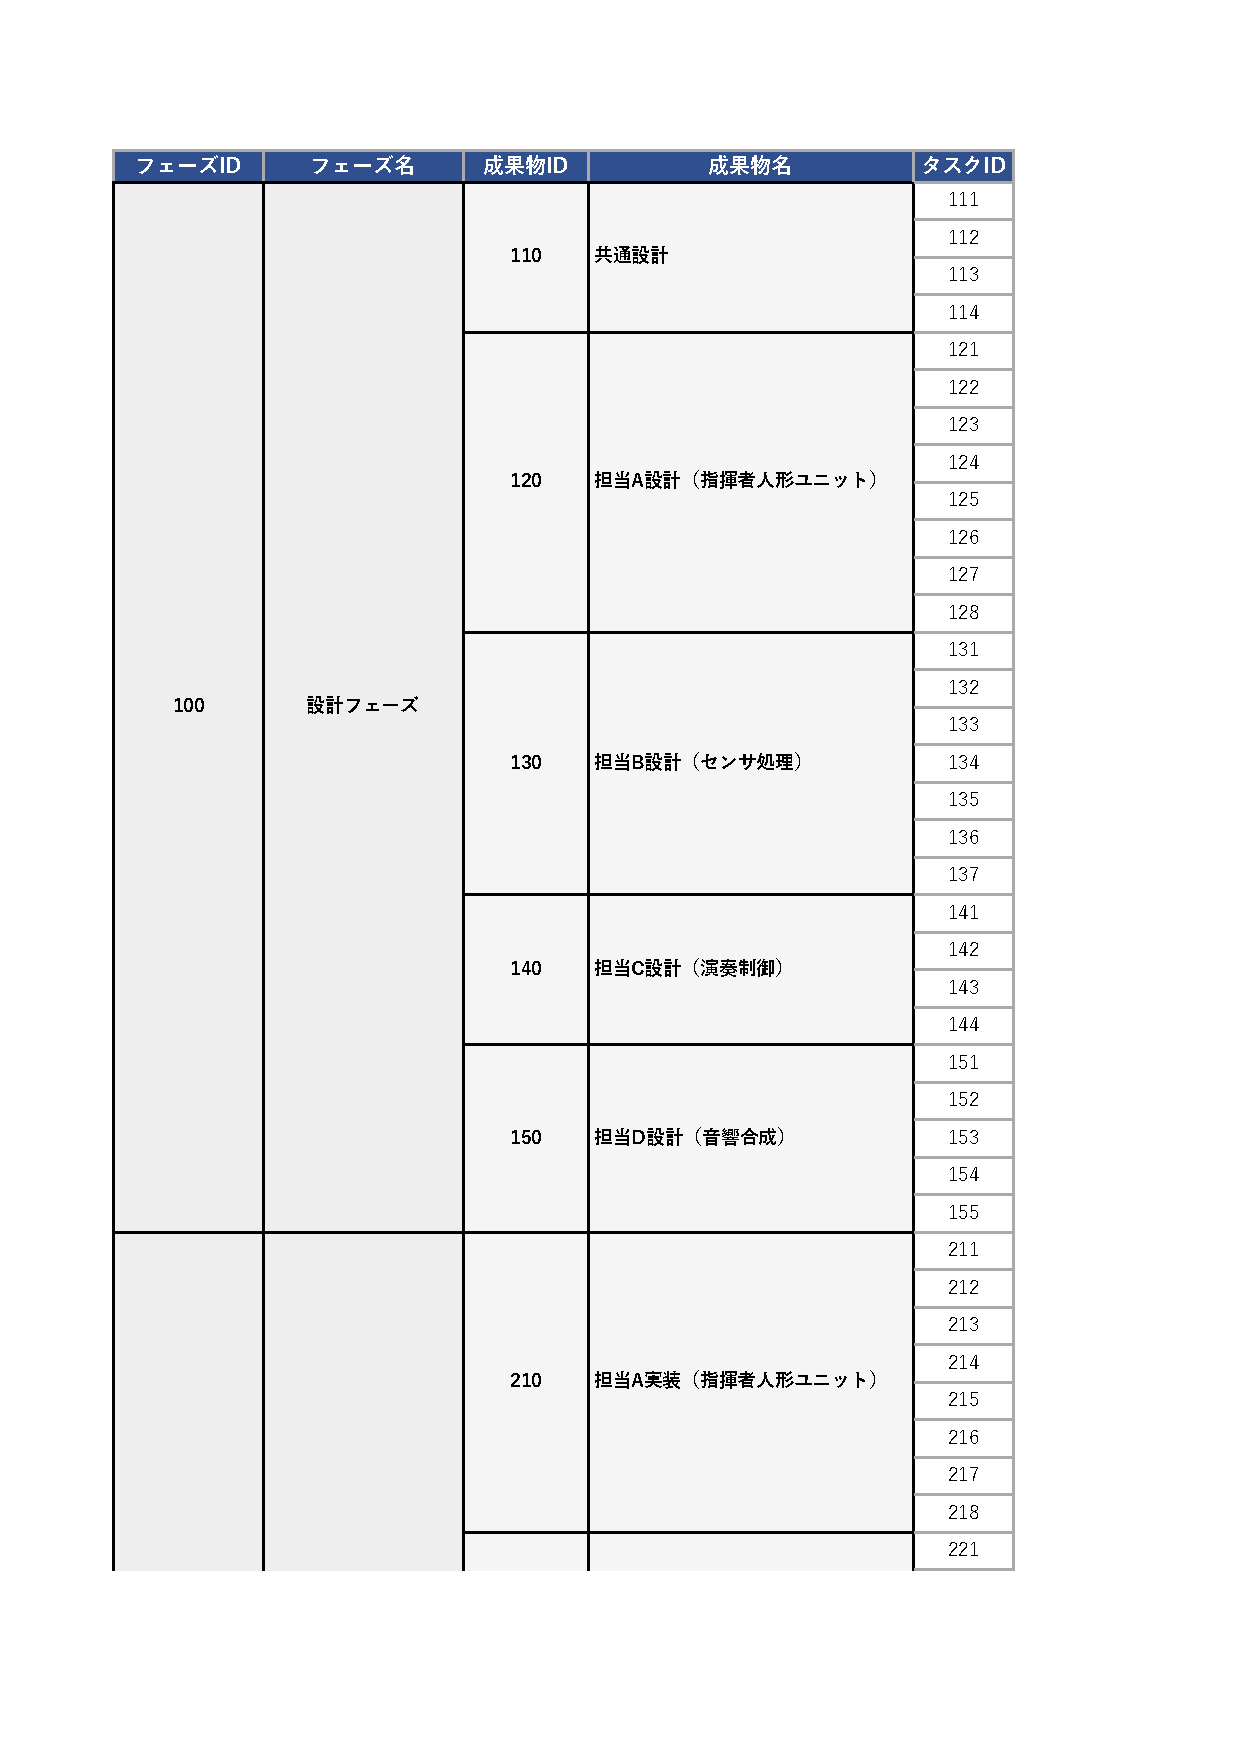
\includegraphics[width=\linewidth]{figures/common/wbs_v2.pdf}
  \caption{作業分解構造（WBS）}
  \label{fig:wbs}
\end{figure}

\subsection{アローダイアグラムとクリティカルパス}
アローダイアグラム（Activity on Arrow形式）を図\ref{fig:arrow}に示す．
各ノードには最早開始日（ES）と最遅開始日（LS）を記載し，
ES = LS となる活動をクリティカルパス（赤矢印）として示す．

\begin{figure}[H]
  \centering
  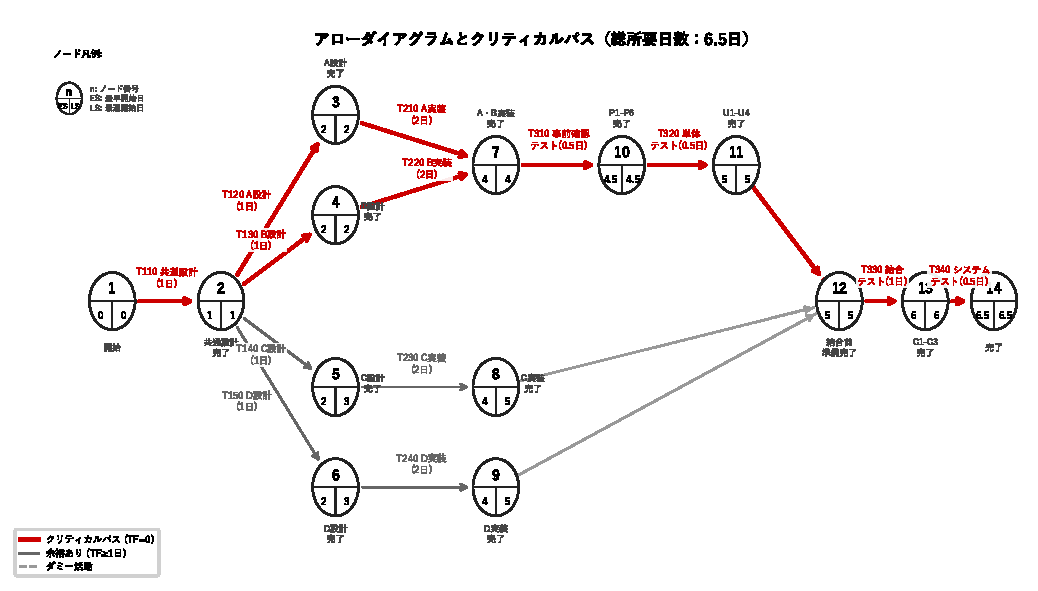
\includegraphics[width=\linewidth]{figures/common/arrow_diagram.pdf}
  \caption{アローダイアグラムとクリティカルパス}
  \label{fig:arrow}
\end{figure}

クリティカルパスは
$①\to②\to③\to⑦\to⑩\to⑪\to⑫\to⑬\to⑭$（担当A実装経由）
および
$①\to②\to④\to⑦\to⑩\to⑪\to⑫\to⑬\to⑭$（担当B実装経由）
の2経路であり，総所要日数は\textbf{6.5日}となる．
担当C・D（T140・T150・T230・T240）は各1日のトータルフロートを有する．

\subsection{役割分担}
WBS（図\ref{fig:wbs}）およびPBSに基づき，各機能およびコンポーネントの設計・実装・テストは以下の担当者に割り当てられている．

\begin{itemize}
  \item \textbf{担当A（指揮者人形ユニット）}：長見・飛田
  \item \textbf{担当B（センサー・観測）}：長野・慶田
  \item \textbf{担当C（演奏制御）}：長山・慶田
  \item \textbf{担当D（音響合成）}：中村・尾添
\end{itemize}

全体に関わる共通設計（WBS 110）や事前確認テスト以降の結合・システムテスト（WBS 300番台の一部）は，全員または関係する担当者が共同で実施する．

\subsection{ガントチャート}
図\ref{fig:gantt}にガントチャートを示す．
フェーズ200（実装）は第6週（5月18日）から各担当が並行して着手する．
第7週（5月25日）は大学のテスト期間に伴うバッファー週（薄橙色）として確保し，
実装作業を一時中断する．
フェーズ300（テスト）は第9週（6月8日）の事前確認テスト（P1--P6）から開始し，
単体テスト（U1--U4），結合テスト（C1--C3）を経て，
第11週（6月22日）のシステムテスト（S1--S3）で完了する．

\begin{figure}[H]
  \centering
  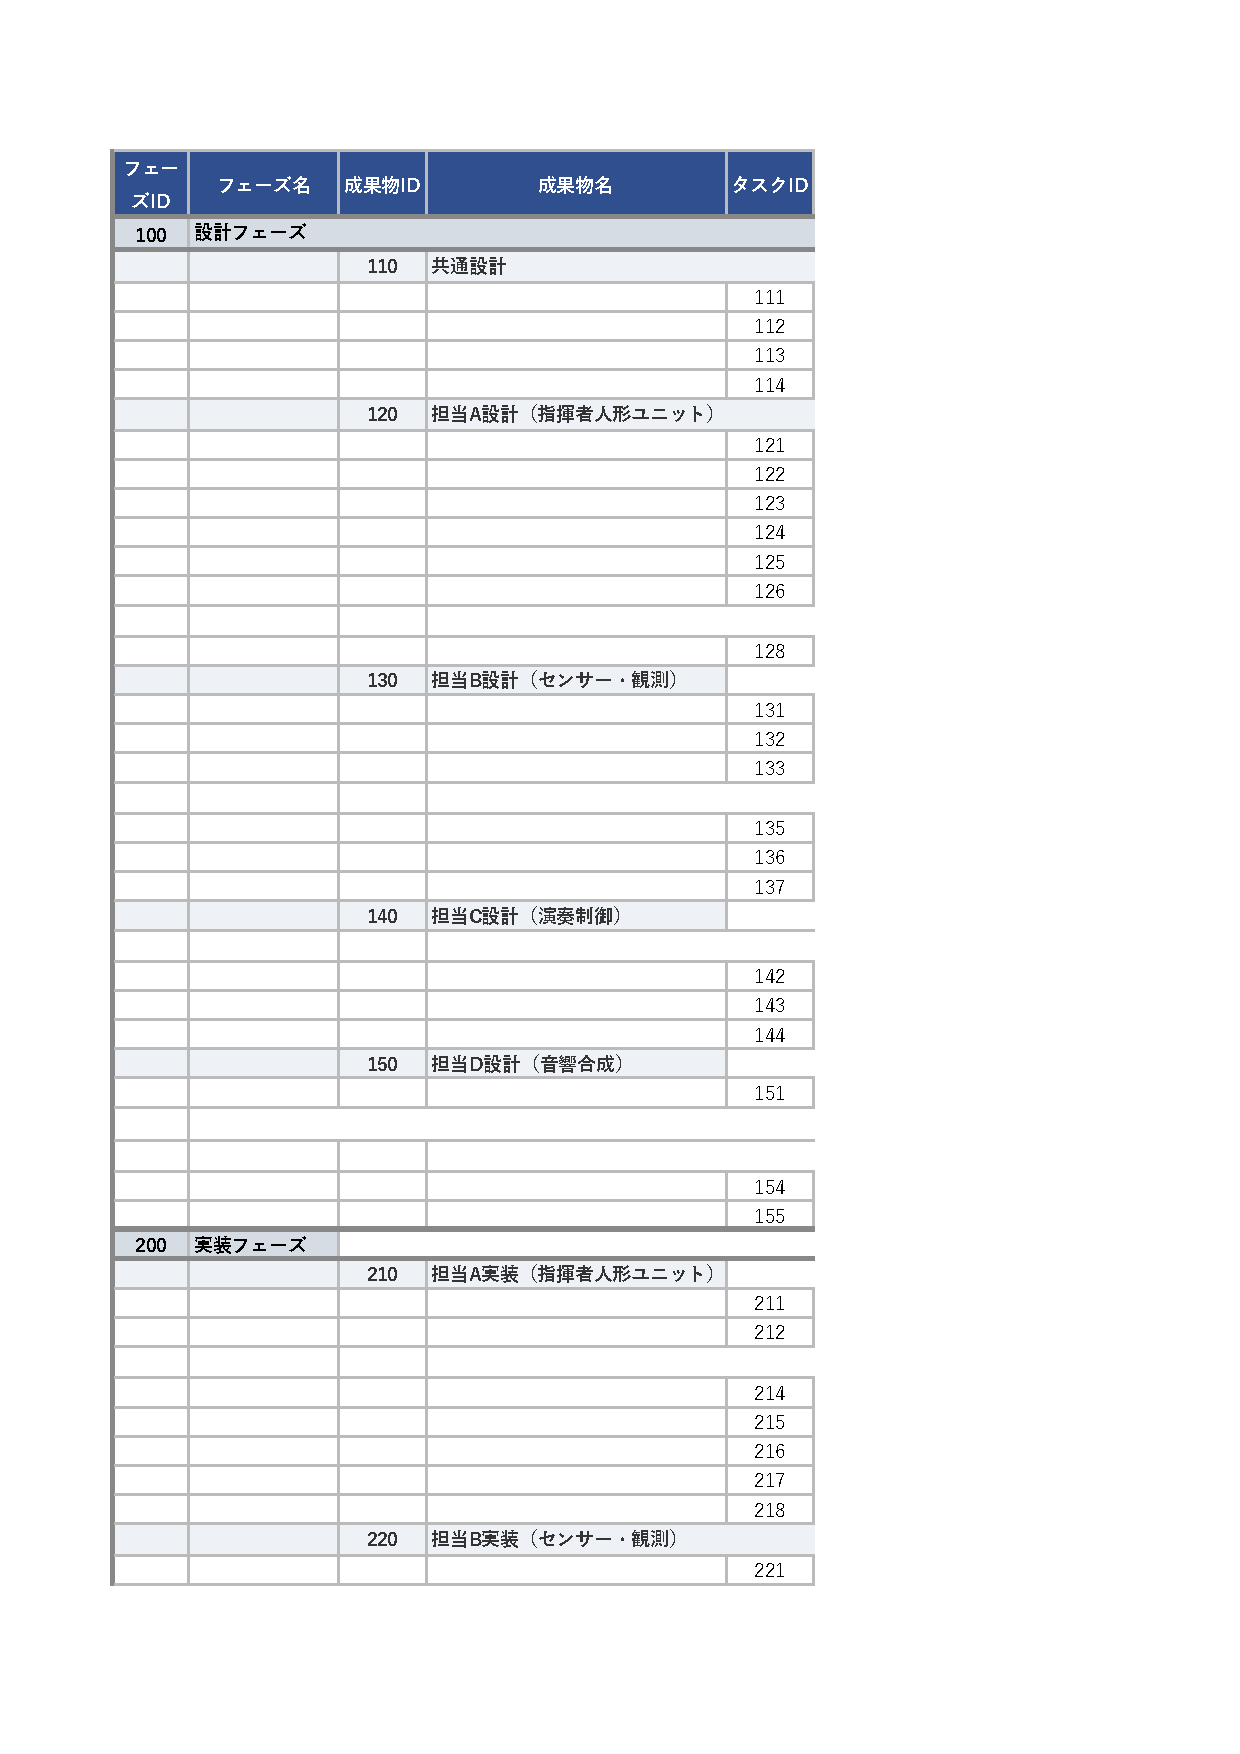
\includegraphics[width=\linewidth]{figures/common/gantt.pdf}
  \caption{ガントチャート}
  \label{fig:gantt}
\end{figure}

% =====================
\section{検証と妥当性確認：V\&V計画}

ハッカソン2テキスト§1.2.5に基づき，MOE → MOP → TPM の順で評価指標を定める．
実運用では順序が逆転し，実装中に TPM を継続監視し，
V\&V によって MOP を確認し，最終的に MOE で受入判定を行う．
本節では各指標の定義・数値目標・設定根拠を示す．
各MOPはスコープ・マネジメント節（§\ref{sec:scope}）で定めたFBSの機能要素に対応して設定している．
各MOPの具体的なテスト手順・判定基準は，第3章（システムの詳細設計）の
各担当節に設けたテスト設計（§3.1〜§3.4）に記述する．

\subsection{プロジェクトの成果物に対する有効指標MOE}

MOE（Measure of Effectiveness：有効指標）は，
ステークホルダ（審査員・聴衆）が成果物の合格・不合格を判定するための指標であり，
受入テストの合否基準に相当する．
本プロジェクトのMOEを表\ref{tab:moe}に示す．

\begin{table}[H]
  \centering
  \caption{MOE一覧}
  \label{tab:moe}
  \begin{tabularx}{\linewidth}{clXl}
    \toprule
    No. & MOE & 内容 & 確認方法 \\
    \midrule
    MOE-1 & 演奏完走 &
      「かえるのうた」5パート輪唱（テンポ変化・フェルマータ含む）を
      最初から最後まで演奏できること &
      実演で確認 \\
    MOE-2 & 指揮追従 &
      指揮者人形のテンポ変化・フェルマータに対して
      演奏が連動していることが視聴覚的に確認できること &
      審査員観察評価 \\
    MOE-3 & 楽器音認識 &
      各パートが意図した楽器（ピアノ・鉄琴・トランペット・
      バス/スネア・ハイハット）の音として聴こえること &
      審査員主観評価 \\
    \bottomrule
  \end{tabularx}
\end{table}

表\ref{tab:moe}に示すように，MOEはMOE-1（演奏完走）・MOE-2（指揮追従）・MOE-3（楽器音認識）の3項目からなる．
MOE-1は本システムの最低限の動作要件であり，演奏が途中で止まることは致命的な失敗にあたるため設定した．
MOE-2は本システムの独自性である「指揮者人形の観測による自律同期」が実際に機能しているかを
聴衆・審査員が知覚できることを確認するために設定した．
MOE-3はProcessingによる音響合成の品質を評価するために設定した．

\subsection{有効指標MOEに対応する性能指標MOP}

MOP（Measure of Performance：性能指標）はMOEを達成するために必要な
システム性能を定量的に示す指標であり，V字モデルの設計段階で定義する．
FBSの各機能に対応する性能要素に対して設定したMOPと，
対応するMOEを表\ref{tab:moe-mop}に示す．

\begin{table}[H]
  \centering
  \caption{MOEとMOPの対応}
  \label{tab:moe-mop}
  \begin{tabularx}{\linewidth}{clX}
    \toprule
    No. & 対応MOE & MOP \\
    \midrule
    1 & MOE-1,2 & フォトトランジスタによる拍検出成功率 \\
    2 & MOE-1,2 & 楽器間の発音タイミング誤差 \\
    3 & MOE-1,2 & テンポ変化後のEMA収束拍数 \\
    4 & MOE-1,2 & 腕停止からフェルマータ状態移行までの拍数 \\
    5 & MOE-3   & 各パートの発音周波数精度 \\
    \bottomrule
  \end{tabularx}
\end{table}

表\ref{tab:moe-mop}に示すMOPはそれぞれMOE-1・MOE-2の達成に関わる技術的な性能要素であり，
各テストフェーズにおいて数値目標として評価する．
具体的な目標値はシステムテスト・結合テスト・単体テストの各節で示す．

\subsection{システムテストで評価する性能指標MOP}

システム全体を統合した状態で評価するMOPを表\ref{tab:mop-sys}に示す．

\begin{table}[H]
  \centering
  \caption{システムテストで評価するMOP}
  \label{tab:mop-sys}
  \begin{tabularx}{\linewidth}{llX}
    \toprule
    No. & 対応FBS機能 & MOP（目標値） \\
    \midrule
    SYS-1 & テンポ推定 &
      テンポ変化後の収束：$\leq 3$拍 \\
    SYS-2 & フェルマータ検出 &
      腕停止からフェルマータ移行：$\leq 1$拍 \\
    SYS-3 & 楽譜進行制御 &
      全区間通し演奏の完走率：$100\,\%$ \\
    \bottomrule
  \end{tabularx}
\end{table}

表\ref{tab:mop-sys}に示す各MOPの目標値の設定根拠を以下に示す．

SYS-1の目標値3拍の根拠を示す．
本楽曲「かえるのうた」は4/4拍子（1小節=4拍）で演奏される．
EMAの更新式は$T_n = \alpha \cdot \Delta t_n + (1-\alpha)\cdot T_{n-1}$であり，
テンポ変化後の残差は$(1-\alpha)^n$で減衰する．
テンポ変化を検出した際の平滑化係数$\alpha=0.5$を用いると，
$n$拍後の残差は$0.5^n$となり，$n=3$のとき$0.5^3=0.125$（87.5\%収束）である．
4/4拍子において，テンポ変化後に1小節未満（$\leq 3$拍）で収束すれば，
次の小節の先頭から新テンポで各楽器が揃って演奏を再開できる．
この「次小節頭で揃う」という音楽的要件と$\alpha=0.5$のEMA特性の両面から，
$\leq 3$拍を目標値とした．

SYS-2の目標値1拍の根拠を示す．
フェルマータは楽譜上で特定の拍に付与される記号であり，
腕停止を検出してから1拍以上経過すると，その拍の音符が余分に発音されて旋律が崩れる．
したがって，腕停止検出から次の拍が来る前にフェルマータ状態へ移行しなければならず，
この楽譜上の制約から$\leq 1$拍を上限として設定した．
フェルマータ検出の具体的な実装はFBS機能F2a4（フェルマータ検出）に対応し，
詳細は担当Bの詳細設計（第3章§3.2）に記述する．

SYS-3の100\%はMOE-1（演奏完走）の定義そのものであり，
システムテストの合格条件として妥協のない値として設定した．

なお，各システムテストの実施手順・判定基準は第3章の各担当詳細設計節に記述する．

\subsection{結合テストで評価する性能指標MOP}

複数の担当成果物を結合した状態で評価するMOPを表\ref{tab:mop-int}に示す．

\begin{table}[H]
  \centering
  \caption{結合テストで評価するMOP}
  \label{tab:mop-int}
  \begin{tabularx}{\linewidth}{llX}
    \toprule
    No. & 対応FBS機能 & MOP（目標値） \\
    \midrule
    INT-1 & テンポ追従演奏 &
      楽器間発音タイミング誤差：$\leq \pm 20\,\mathrm{ms}$ \\
    INT-2 & テンポ追従演奏 &
      Arduino→Processing転送遅延：$\leq 50\,\mathrm{ms}$ \\
    INT-3 & 輪唱オフセット制御 &
      輪唱オフセット誤差：$\leq \pm 1$拍 \\
    \bottomrule
  \end{tabularx}
\end{table}

表\ref{tab:mop-int}に示す各MOPの設定根拠を以下に示す．
INT-1の目標値$\pm 20\,\mathrm{ms}$は，人間が音楽的なタイミングのズレを知覚できる
閾値（先行研究では概ね$20\sim30\,\mathrm{ms}$\cite{sudo2007,kawase}）の下限値を採用した．
INT-2の目標値$50\,\mathrm{ms}$の根拠を示す．
115200\,bpsのシリアル通信では，スタート・データ8bit・ストップビットを含む1バイト=10bitを送信する．
3バイトパケットの純粋な転送時間は$\frac{3 \times 10}{115200} \approx 0.26\,\mathrm{ms}$である．
これにProcessing側のバッファ読み取り間隔（典型10\,ms未満）を加えても実測値は数ms程度であり，
$50\,\mathrm{ms}$は十分な余裕を持った上限値である．
また，各楽器ユニットで遅延が一定であれば遅延補正値で吸収できるため，絶対値よりも安定性が重要である．

INT-3の目標値$\pm 1$拍の根拠を示す．
輪唱は各パートが一定拍数ずれて同じ旋律を演奏する構造であり，
オフセットが$\pm 1$拍以上ずれると隣接パートの音符と重なり旋律が崩れる．
したがって輪唱として成立する最小単位である「1拍」をそのまま上限として設定した．

なお，結合テストの具体的な実施手順・タイムスタンプ計測方法は，
担当B・Cの詳細設計（第3章§3.2・§3.3）に記述する．

\subsection{単体テストで評価する性能指標MOP}

各担当成果物を単独で評価する単体テストのMOPを表\ref{tab:mop-unit}に示す．

\begin{table}[H]
  \centering
  \caption{単体テストで評価するMOP}
  \label{tab:mop-unit}
  \begin{tabularx}{\linewidth}{lX}
    \toprule
    No. & MOP（目標値） \\
    \midrule
    UNIT-1 & 拍検出成功率：$\geq 95\,\%$ \\
    UNIT-2 & 距離計算誤差：$\leq \pm 3\,\mathrm{cm}$ \\
    UNIT-3 & EMA通常演奏時（$\alpha=0.2$）の収束：$\leq 13$拍 \\
    UNIT-4 & NOTE\_ON送信タイミング誤差：$\leq \pm 10\,\mathrm{ms}$ \\
    UNIT-5 & 発音周波数精度：目標周波数の$\pm 1\,\mathrm{Hz}$以内 \\
    UNIT-6 & BPM追従誤差：$\leq \pm 5\,\mathrm{bpm}$ \\
    UNIT-7 & ストローク変動：$\leq \pm 2\,\mathrm{mm}$ \\
    \bottomrule
  \end{tabularx}
\end{table}

表\ref{tab:mop-unit}に示す各MOPの設定根拠を以下に示す．

UNIT-1の目標値95\%の根拠を示す．
検出失敗率を$p = 1 - 0.95 = 0.05$とすると，3拍連続で失敗する確率は
$p^3 = 0.05^3 = 1.25 \times 10^{-4}$（約0.013\%）である．
フォールバック処理は3拍連続未検出で発動するため，
検出成功率95\%を維持すればフォールバックがほぼ発動しないことが保証される．

UNIT-2の目標値$\pm 3\,\mathrm{cm}$の根拠を示す．
フェルマータ検出は絶対距離ではなく腕の「変化量」$\Delta d$で判定するため，
絶対距離の精度要件は緩やかである．
センサー出力電圧$V$から距離$d$を推定する近似式$d = 27.728 \times V^{-1.2045}$において，
ArduinoのAD変換（10bit，5\,V系）の量子化誤差$\Delta V \approx 5/1024 \approx 4.9\,\mathrm{mV}$を伝搬させると，
$d \approx 30\,\mathrm{cm}$付近での距離誤差は数mm〜数cm程度となる．
この誤差範囲を包含する上限として$\pm 3\,\mathrm{cm}$を設定した．

UNIT-3の目標値13拍の根拠を示す．
$\alpha=0.2$のEMAが95\%収束（残差$\leq 5\%$）するのに必要な拍数は，
$(1-\alpha)^n \leq 0.05$を解いて
$n \geq \frac{\ln 0.05}{\ln(1-\alpha)} = \frac{\ln 0.05}{\ln 0.8} \approx 13.4$拍，
切り上げで14拍となる．
14拍以内に収束することを確認するため，余裕を1拍見て13拍を確認目標とした．

UNIT-4の目標値$\pm 10\,\mathrm{ms}$の根拠を示す．
楽器間タイミング誤差（INT-1：$\pm 20\,\mathrm{ms}$）は，
各楽器の送信誤差が独立に重なった合計で生じる．
最悪ケースで2つの楽器が逆方向に最大誤差を持つと，
$(\pm 10) - (\pm 10) = \pm 20\,\mathrm{ms}$となる．
よって，各楽器単体の誤差をINT-1の半分である$\pm 10\,\mathrm{ms}$以内に抑えることでINT-1を満たせる．

UNIT-5の目標値$\pm 1\,\mathrm{Hz}$は，音楽的に許容されるピッチのずれ（約$\pm 5\,\mathrm{cent}$，
A4=440\,Hzで約$\pm 1.3\,\mathrm{Hz}$\cite{jnd1974}）に対して余裕を持たせた値である．

UNIT-6の目標値$\leq \pm 5\,\mathrm{bpm}$の根拠を示す．
80\,bpmを基準テンポとすると，1拍の周期は$60/80 = 750\,\mathrm{ms}$である．
人間がテンポ変化を知覚できる閾値は一般に約3〜6\%とされており，
80\,bpmの6\%は$80 \times 0.06 = 4.8\,\mathrm{bpm}$である．
この値を切り上げた$\pm 5\,\mathrm{bpm}$を，聴衆が追従と判断できる上限として設定した．

UNIT-7の目標値$\leq \pm 2\,\mathrm{mm}$の根拠を示す．
指揮者人形のストローク幅はEMA（担当B）が計算する「振り幅」に対応し，
ストローク変動が大きいとBPM推定の誤差（UNIT-6）に直接影響する．
UNIT-6の目標値$\leq \pm 5\,\mathrm{bpm}$を80\,bpmにおける1拍周期の変動量に換算すると，
$\Delta T = 60/80 - 60/85 \approx 44\,\mathrm{ms}$であり，
これを引き起こすストローク誤差は機構設計（担当A詳細設計§3.1）の寸法から$\pm 2\,\mathrm{mm}$以内と見積もられる．

各単体テストの具体的な実施手順は，第3章の各担当詳細設計節
（担当A：§3.1，担当B：§3.2，担当C：§3.3，担当D：§3.4）のテスト設計に記述する．

\subsection{プロジェクト中に監視する技術性能指標TPM}

TPM（Technical Performance Measure：技術性能指標）は，開発・実装中に
継続的に測定・報告する定量的指標であり，技術的リスクの早期発見を目的とする．
MOPのうち特にシステム完成時の性能に大きく影響し，
実装の早い段階から測定できる項目を選定した．
TPM一覧を表\ref{tab:tpm}に示す．

\begin{table}[H]
  \centering
  \caption{TPM一覧}
  \label{tab:tpm}
  \begin{tabularx}{\linewidth}{lX}
    \toprule
    No. & TPM（監視値・許容範囲） \\
    \midrule
    TPM-1 & 距離計算誤差：$\leq \pm 3\,\mathrm{cm}$ \\
    TPM-2 & 拍検出成功率：$\geq 95\,\%$ \\
    TPM-3 & Arduino→Processing転送遅延：$\leq 50\,\mathrm{ms}$ \\
    TPM-4 & EMA（$\alpha=0.2$）テンポ収束拍数：$\leq 13$拍 \\
    TPM-5 & 指揮者人形が追従できる最大BPM：$\geq 104\,\mathrm{bpm}$ \\
    TPM-6 & テンポ予測誤差（予測拍時刻と実測拍時刻の差）：$\leq 1\,\mathrm{ms}$ \\
    \bottomrule
  \end{tabularx}
\end{table}

\subsection{TPMの監視体制}

表\ref{tab:tpm-monitor}に，各TPMの監視方法を示す．
監視方法の詳細（使用機材・記録フォーマット）は第3章各担当詳細設計節のテスト設計に記述する．

\begin{table}[H]
  \centering
  \caption{TPM監視体制}
  \label{tab:tpm-monitor}
  \begin{tabularx}{\linewidth}{lX}
    \toprule
    TPM & 監視方法 \\
    \midrule
    TPM-1 & 既知距離での実測値と近似式の計算値を比較し誤差を記録する \\
    TPM-2 & メトロノームに合わせた指揮動作でフォトTrの検出率をシリアルモニタで計測する \\
    TPM-3 & Arduino側の送信タイムスタンプとProcessing側の受信タイムスタンプの差分を計測・記録する \\
    TPM-4 & 既知BPMのシミュレーションデータを入力してEMAの収束拍数を計測する \\
    TPM-5 & 指定BPMで指揮者人形を動作させ，脱調・遅延の有無をシリアルモニタで確認する \\
    TPM-6 & シリアルモニタで予測拍時刻と実測拍時刻の差を100回計測し，平均誤差を記録する \\
    \bottomrule
  \end{tabularx}
\end{table}

% =====================
\section{資源・調達管理}

\subsection{人的資源}

本プロジェクトの人的資源は7名のメンバーで構成される．
各メンバーは担当A〜Dのいずれかに所属し，設計・実装・テストの全工程を通じてその担当領域を主体的に推進する（表\ref{tab:human-resource}）．

\begin{table}[H]
  \centering
  \caption{人的資源一覧}
  \label{tab:human-resource}
  \begin{tabularx}{\linewidth}{llX}
    \toprule
    担当 & メンバー & 主な責務 \\
    \midrule
    A（指揮者人形ユニット） & 長見・飛田 & 人形機構組み立て，LED・サーボ駆動回路，サーボ制御SW \\
    B（センサー・観測）     & 長野・慶田 & センサー配線，センサーISR・EMAテンポ推定・状態機械SW \\
    C（演奏制御）           & 長山・慶田 & 楽譜配列作成，拍検出・楽譜進行・シリアル送信SW \\
    D（音響合成）           & 中村・尾添 & 音色定義データ，音色合成エンジン・エフェクトProcessing SW \\
    \bottomrule
  \end{tabularx}
\end{table}

共通設計（WBS 110）および結合・システムテスト（WBS 330・340）は全員または関係担当者が共同で実施し，特定担当に過負荷が集中しないよう調整する．

\subsection{機材・調達計画}

本プロジェクトで必要なハードウェア機材を表\ref{tab:procurement}に示す．
実験室に常備されている機材（既備）は追加調達不要とし，不足分のみを授業実施機関に申請または自費で調達する．

\begin{table}[H]
  \centering
  \caption{機材・調達計画}
  \label{tab:procurement}
  \begin{tabularx}{\linewidth}{Xlcc}
    \toprule
    機材名 & 用途 & 数量 & 調達区分 \\
    \midrule
    Arduino Uno R4 WiFi & 指揮者・観測・演奏各制御 & 6 & 既備 \\
    サーボモータ（SG92R） & 指揮者人形の腕往復動作 & 1 & 既備 \\
    赤外線距離センサ（Sharp GP2Y0A21YK） & 腕位置連続観測 & 5 & 既備 \\
    フォトトランジスタ & 指揮者LED発光の拍検出 & 5 & 既備 \\
    高輝度LED（赤外線） & 指揮者側拍通知光源 & 2 & 既備 \\
    抵抗・コンデンサ類 & 各回路の定数設定 & 適量 & 既備 \\
    ブレッドボード・ジャンパ線 & プロトタイプ配線 & 適量 & 既備 \\
    スピーカ（パッシブ）& Processing音声出力 & 5 & 既備 \\
    工作材料（段ボール・スポンジ等） & 人形機構・遮光チャンバー筐体 & 適量 & 申請調達 \\
    PC（Processing実行用） & 音響合成・シリアル受信 & 6 & 持ち込み \\
    \bottomrule
  \end{tabularx}
\end{table}

調達が必要な物品（工作材料）は第5週（5月11日）までに申請を完了し，
第6週（5月18日）の実装開始に間に合うよう手配する．
電子部品は実験室常備品で賄えない場合のみ，担当Aが第5週中に代替品の確認および申請を行う．

\subsection{開発環境}

本プロジェクトで使用するソフトウェア開発環境を以下に示す．
いずれも無償利用可能なツールであり，追加ライセンス費用は発生しない．

\begin{itemize}
  \item \textbf{Arduino IDE 2.x}：ArduinoのSW開発・書き込み（担当A・B・C）
  \item \textbf{Processing 4.x}：音響合成SWの開発・実行（担当D）
  \item \textbf{draw.io}：FBS・PBS・WBS図の作成・管理（全員）
  \item \textbf{Git / GitHub}：ソースコードのバージョン管理（全員）
  \item \textbf{LuaLaTeX / jlreq}：本計画書・設計書のドキュメント作成（全員）
\end{itemize}

% =====================
\section{リスク管理}

\subsection{リスクの識別と評価}

プロジェクト遂行上のリスクを識別し，発生確率（H/M/L）と影響度（H/M/L）の組み合わせでリスクレベルを評価した結果を表\ref{tab:risk}に示す．

\begin{table}[H]
  \centering
  \caption{リスク一覧と評価}
  \label{tab:risk}
  \begin{tabularx}{\linewidth}{clXcc}
    \toprule
    No. & リスク名 & 内容 & 確率 & 影響 \\
    \midrule
    R-1 & センサー精度不足 &
      フォトTr・赤外線センサが要求精度（UNIT-1：95\%，UNIT-2：$\pm3\,$cm）を
      達成できず，拍検出やフェルマータ検出が不安定になる &
      M & H \\
    R-2 & サーボ最大BPM不足 &
      SG90のトルク・応答速度が不足し，目標最大BPM（TPM-5：104\,bpm）で
      脱調または動作遅延が生じる &
      M & M \\
    R-3 & EMAチューニング失敗 &
      $\alpha$の値が適切に調整できず，テンポ収束（SYS-1：$\leq3$拍）や
      フェルマータ検出（SYS-2：$\leq1$拍）が達成できない &
      M & H \\
    R-4 & 通信遅延超過 &
      Arduino→Processing間のシリアル遅延がINT-2（$\leq50\,$ms）を
      超え，発音タイミングがずれる &
      L & M \\
    R-5 & 機材調達遅延 &
      3Dプリント材料等の申請承認が遅れ，第6週の実装開始が遅延する &
      L & H \\
    R-6 & スケジュール圧迫 &
      各担当の実装が第8週までに完了せず，第9週からのテストフェーズが
      縮小または中止になる &
      M & H \\
    R-7 & 遮光チャンバー性能不足 &
      外乱光によりフォトTrが誤検出し，拍検出成功率（UNIT-1）が低下する &
      M & M \\
    \bottomrule
  \end{tabularx}
\end{table}

\subsection{リスク対応計画}

表\ref{tab:risk}で識別した各リスクに対する対応策を表\ref{tab:risk-response}に示す．

\begin{table}[H]
  \centering
  \caption{リスク対応計画}
  \label{tab:risk-response}
  \small
  \begin{tabularx}{\linewidth}{clXX}
    \toprule
    No. & リスク名 & 対応策（軽減/回避/受容） & トリガー条件 \\
    \midrule
    R-1 & センサー精度不足 &
      【軽減】事前確認テスト（P1--P3）でセンサー単体精度を第9週頭に検証し，
      不足時はセンサー取り付け位置・遮光調整または閾値再設定を行う &
      UNIT-1$<$95\%またはUNIT-2$>\pm3\,$cm \\
    R-2 & サーボ最大BPM不足 &
      【軽減】事前確認テスト（P4--P5）でサーボ最大BPMを実測し，
      不足時は腕のストローク角度を縮小して応答速度を確保する &
      TPM-5$<$104\,bpm \\
    R-3 & EMAチューニング失敗 &
      【軽減】シミュレーションデータによる単体テスト（U1）でEMAの
      収束特性を事前検証し，$\alpha$を段階的に調整して目標範囲内に収める &
      収束拍数$>$3拍またはフェルマータ移行$>$1拍 \\
    R-4 & 通信遅延超過 &
      【受容・軽減】115200\,bpsの遅延は理論上1\,ms未満であり発生確率は低い．
      万一超過した場合はバッファ読み取り処理をPollingからイベント駆動に変更する &
      TPM-3$>$50\,ms \\
    R-5 & 機材調達遅延 &
      【回避】第5週（5月11日）中に申請を完了し，承認が遅れる場合は
      手持ちの材料で代替した簡易筐体を先行して製作する &
      第6週開始時点で材料未着 \\
    R-6 & スケジュール圧迫 &
      【軽減】第7週のバッファー週を活用して遅延分を吸収する．
      それでも遅延が残る場合は，未完了タスクをテストフェーズ前半（第9週）に繰り越し，
      テストスコープを縮小して対応する &
      第8週末時点で実装完了率$<$90\% \\
    R-7 & 遮光チャンバー性能不足 &
      【軽減】遮光チャンバーに黒色テープ・フォームを追加して外乱光を遮断する．
      それでも改善しない場合はフォトTrをシールドケースに封入する &
      屋内通常照明下でUNIT-1$<$95\% \\
    \bottomrule
  \end{tabularx}
\end{table}

\subsection{リスク監視体制}

各担当は週次のミーティング（授業時間内）にTPMの計測結果を報告し，
表\ref{tab:risk}のトリガー条件に抵触したリスクが発生した場合は
その場で対応策の着手を決定する．
リスクレベルがH×H（高確率かつ高影響）に達した場合は全員でスコープの再確認を行い，
MOE-1（演奏完走）の達成を最優先として成果物を取捨選択する．


% =============================================================
\chapter{システムの基本設計}

設計書は作成する成果物によって変化します．適宜修正して利用してください．

% ===================== 担当A =====================
\section{担当A — 指揮者人形・センサ機構}

\subsection{機能一覧}
担当Aでは，楽器ユニット（子機）が演奏を同期させるための指揮者人形ユニット（親機）を開発を担当する．
指揮者人形ユニットは，Arduinoオーケストラにおいて演奏の開始・停止の合図を出し，一定のテンポで腕を振ることで，各楽器ユニット（子機）が同期させるための基準となる役割を担う．\par
本ユニットが担う主な機能は以下の通りである．

\begin{itemize}
    \item \textbf{テンポ提示機能}\\
    腕（反射板）を一定周期で滑らかに往復運動させ，1往復を1拍としてオーケストラ全体のテンポを提示する．

    \item \textbf{拍の同期機能}\\
    腕が最前点に到達した瞬間に，反射板に搭載したLEDを短時間点灯させる．子機は「LEDの光」と「反射板までの距離の変動」の２つの物理的変化を観測することで，通信に頼らず性格に拍を同期する．

    \item \textbf{演奏状態の表現機能}\\
    「待機」「予備拍」「演奏中」「フェルマータ」「演奏停止」の各状態を持ち，状態に応じた動作の変化によって演奏の展開を表現する．

    \item \textbf{外部制御・情報表示機能}\\
    PC上の制御アプリケーションからシリアル通信経由で制御コマンド（START・STOP・FERMATA）を受信する．また．現在の演奏状態を本体のLCDディスプレイに表示し，ユニット単体での状況把握を可能にする．
\end{itemize}

\subsection{システム構成図}
本システムは，ユーザが操作するPC側の制御アプリケーション（Processing），制御と状態管理を担うマイクロコントローラ（Arduino Uno R4 WiFi），および動作と状態提示を行う各出力デバイスによって構成される．
PCからの制御コマンド受信，FspTimerを用いた割り込み処理，およびマイクロ秒単位でのデバイス同期のフローを含む，システム全体の構成図を以下の図\ref{tantoA:system}に示す．

\begin{figure}[H]
    \centering
    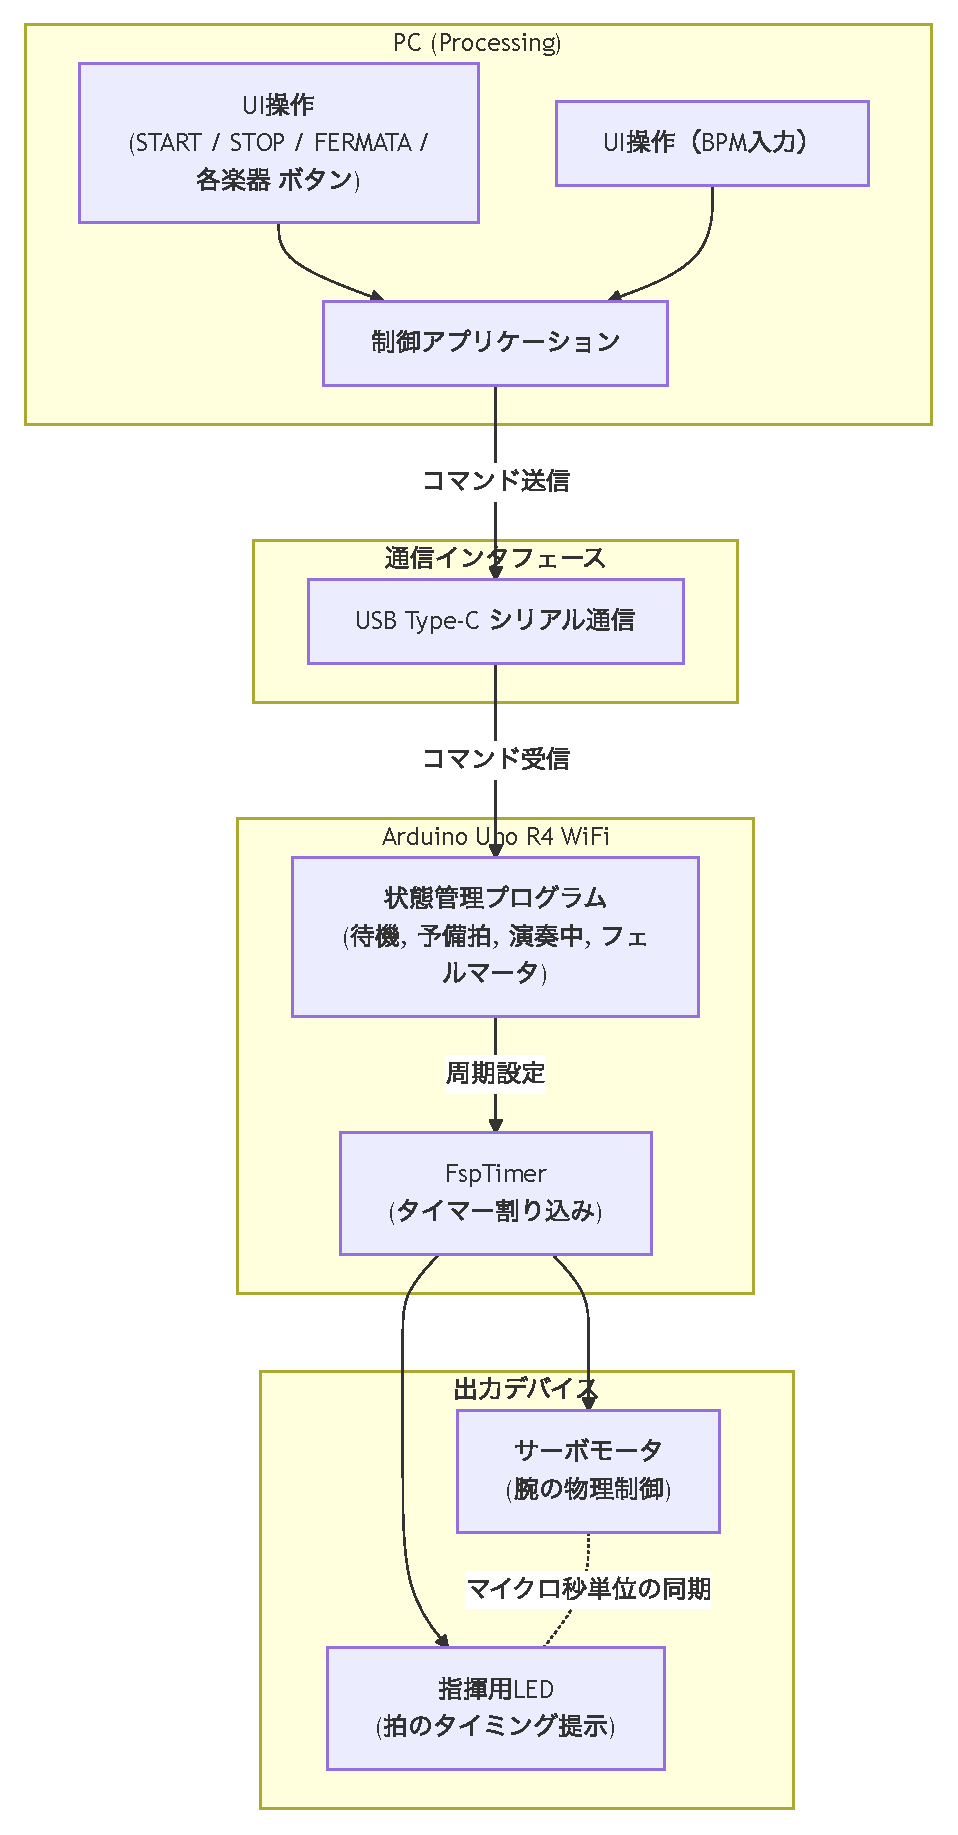
\includegraphics[width=8cm]{figures/tantoA/configuration.pdf}
    \caption{システム構成図}
    \label{tantoA:system}
\end{figure}

\subsection{操作インターフェース設計}
本システムでは，信号入力用の制御アプリケーション（Processingを用いて構築）を介して指揮者人形ユニットの操作を行う．
ユーザインターフェースには，図\ref{tantoA:user}に示すように「START」「STOP」「FERMATA」の各制御ボタンを配置する．
ユーザがPC上でこれらのボタンをクリックすることで，USB Type-Cを用いたシリアル通信を介して，対応する信号がArduinoへ送信される．

\begin{figure}[H]
    \centering
    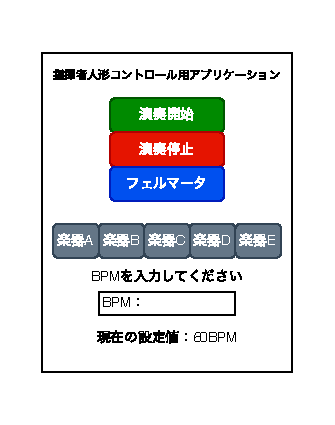
\includegraphics[width=5cm]{figures/tantoA/UI_image.pdf}
    \caption{ユーザーインターフェース表示案}
    \label{tantoA:user}
\end{figure}

\subsection{状態遷移図}
本システムにおける状態遷移図を以下の図\ref{tantoA:flowchart}に示す.

\begin{figure}[H]
    \centering
    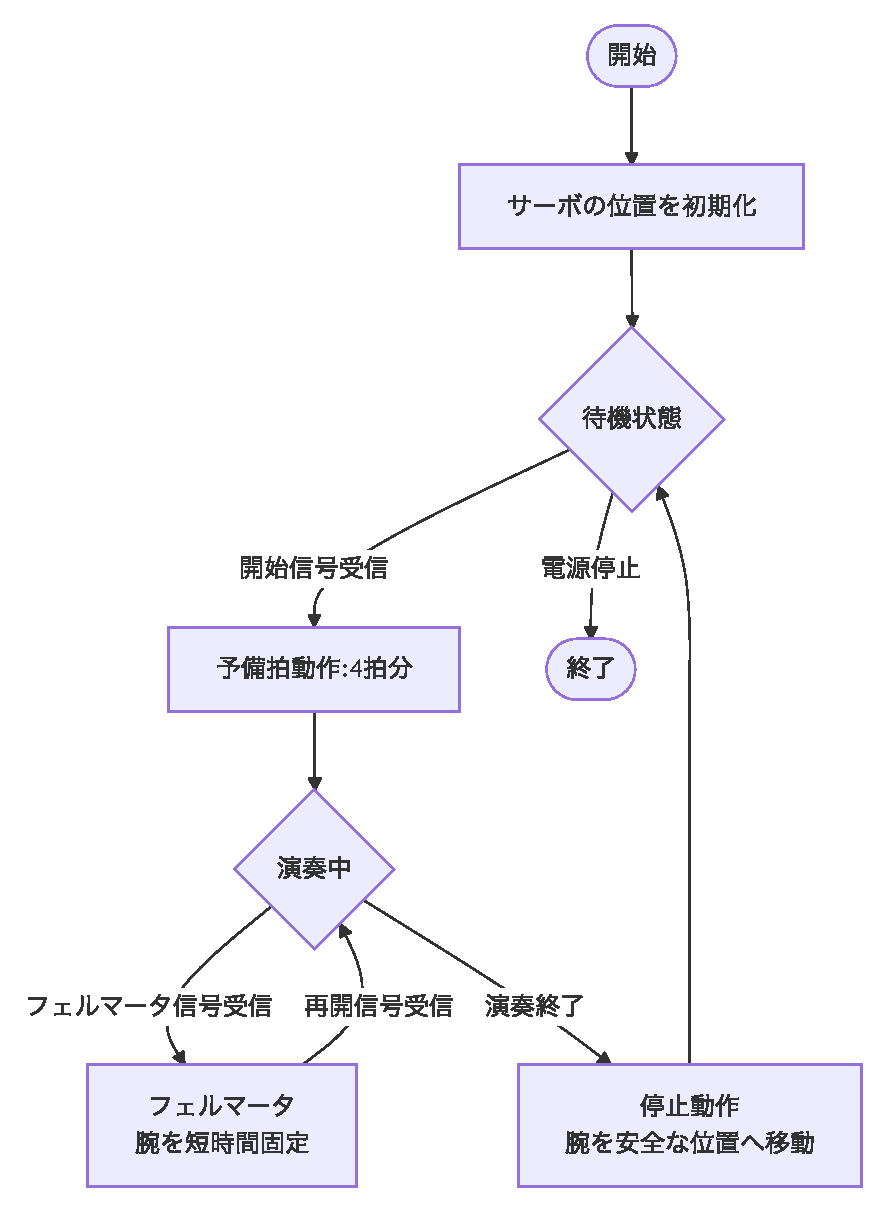
\includegraphics[width=8cm]{figures/tantoA/conductor.pdf}
    \caption{指揮者人形ユニットにおける状態遷移図}
    \label{tantoA:flowchart}
\end{figure}



\section{担当B — センサ処理・状態機械}

\subsection{機能一覧}

担当Bでは，楽器ユニットにおけるセンサー処理およびArduinoによる制御を担当する．
本システムでは，指揮者ロボットの腕に搭載されたLEDをフォトトランジスタで検出し，
その情報をもとに演奏タイミングを決定する．

各楽器ユニットは独立して動作しており，
通信を用いることなく指揮者の動きに追従して同期演奏を行う．

各楽器ユニットは，あらかじめ内部に楽譜データを保持しており，
取得した拍情報に基づいて順次演奏を行う．
各楽器の演奏開始タイミングは，親機のカラーLEDをカラーセンサで識別することで決定される．
各楽器ユニットはあらかじめ自楽器に対応する色名を設定しており，
その色を拍タイミングで検出した時点で演奏を開始する．

担当Bが提供する主な機能を以下に示す．

\begin{itemize}
  \item フォトトランジスタによる拍タイミングの検出（デジタル入力）
  \item EMA（指数移動平均）によるテンポ推定
  \item カラーセンサによる演奏開始キュー（色）の判別
  \item 状態機械による演奏状態の管理
  \item 担当Cへの拍タイミング・状態情報の共有
\end{itemize}

\subsection{システム構成図}

図\ref{fig:system_B} にシステム全体の構成を示す．

\begin{figure}[H]
\centering
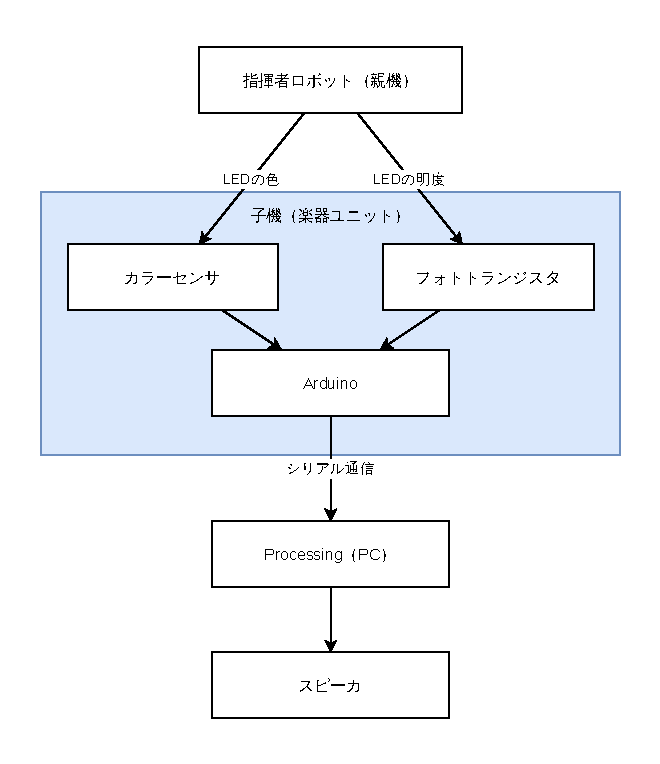
\includegraphics[width=0.8\linewidth]{figures/tantoB/B_system.pdf}
\caption{システム構成図}
\label{fig:system_B}
\end{figure}

\subsection{操作インターフェース設計}

本システムでは，指揮者ロボットの腕の動きが操作インターフェースとなる．
各楽器ユニットはフォトトランジスタとカラーセンサを通じて指揮者の動きを観測することで，
ユーザーが個別の楽器を操作することなく演奏タイミングを制御できる．

\subsubsection*{計測方法}
本システムでは，フォトトランジスタとカラーセンサの2種類のセンサを用いて
指揮者の動きを計測する．
フォトトランジスタにより拍のタイミングを検出し，
カラーセンサにより演奏開始キューの色を判別することで，
各楽器の演奏開始タイミングを決定する．

\subsubsection*{拍の検出（フォトトランジスタ）}
フォトトランジスタは，受光量に応じて出力が変化する素子であり，
デジタルピンから \texttt{HIGH} / \texttt{LOW} を読み取ることで受光量を取得する．
指揮者の腕が振り下ろされた瞬間に点灯するLEDの光を受光すると出力が \texttt{HIGH} に切り替わる．
この立ち上がりエッジを毎ループのポーリングで検出することで拍の基準タイミングを取得する．
チャタリングおよびノイズ誤検出を防ぐため，前回の検出から200\,ms以内の再検知は無視する（300\,BPM相当）．

\subsubsection*{演奏開始キューの判別（カラーセンサ）}
演奏者がProcessing GUIから任意の順序で各楽器を指定することで，
親機のカラーLEDが対応する色を発光する．
カラーセンサ（AE\_S13683\_LED）は拍を検出したタイミングで一発測定を行い，
取得したRGB値をコサイン類似度で色名に変換する（表\ref{tab:detect_colors}）．
各楽器ユニットはあらかじめ自楽器に対応する色名を \texttt{PLAY\_COLOR\_NAME} に設定しており，
検出した色が一致した時点で演奏開始フラグ（\texttt{isPlaying}）を立て，
以降の拍タイミングで楽譜の送信を開始する．

楽器IDとカラーLEDの対応を表\ref{tab:color_map}に示す．

\begin{table}[H]
\centering
\caption{判別対象の色一覧}
\label{tab:detect_colors}
\begin{tabular}{lrrr}
\hline
色名 & 参照R（正規化） & 参照G（正規化） & 参照B（正規化） \\\hline
Red     & 0.975 & 0.222 & 0.017 \\
Green   & 0.130 & 0.957 & 0.261 \\
Blue    & 0.088 & 0.406 & 0.910 \\
Yellow  & 0.524 & 0.828 & 0.203 \\
Cyan    & 0.082 & 0.754 & 0.653 \\
Magenta & 0.519 & 0.371 & 0.770 \\
White   & 0.364 & 0.717 & 0.596 \\\hline
\end{tabular}
\end{table}

\begin{table}[H]
\centering
\caption{楽器IDとカラーLEDの対応（\texttt{PLAY\_COLOR\_NAME} 設定値）}
\label{tab:color_map}
\begin{tabular}{ccc}
\hline
楽器ID & 楽器名 & \texttt{PLAY\_COLOR\_NAME} \\\hline
楽器1 & ハイハット・シンバル & Red（赤） \\
楽器2 & バス・スネア         & Green（緑） \\
楽器3 & 鉄琴                 & Blue（青） \\
楽器4 & ピアノ               & Yellow（黄） \\
楽器5 & トランペット         & White（白） \\\hline
\end{tabular}
\end{table}

\subsubsection*{テンポ推定}
フォトトランジスタによって取得した連続する2拍の検出時刻から
拍間隔$\Delta t_n$を求め，EMAによって拍間隔推定値$T_n$を更新する．

\begin{equation}
  T_n = \alpha \cdot \Delta t_n + (1 - \alpha) \cdot T_{n-1}
\end{equation}

ここで$\alpha$はEMA係数（$0 < \alpha < 1$）であり，$\alpha = 0.2$とする．
測定拍間隔$\Delta t_n$と前回推定拍間隔$T_{n-1}$の誤差率が
閾値$\delta$（デフォルト10\%）を超えた場合はEMAをバイパスして$\Delta t_n$を直接採用し，
急激なテンポ変化に素早く追従する．なお，この誤差率チェックは予備振り状態（PREBEAT）では行わず，
常にEMAを適用する．

\begin{equation}
  \text{誤差率} = \frac{|\Delta t_n - T_{n-1}|}{T_{n-1}} \times 100 \quad [\%]
\end{equation}

次の拍の予測時刻$t_{\text{next}}$は以下の式で計算する．

\begin{equation}
  t_{\text{next}} = t_{\text{beat}} + T_n
\end{equation}

\subsection{状態遷移図}

本システムでは，演奏状態を以下の3状態で管理する．

\begin{itemize}
  \item 停止状態（IDLE）：演奏を行わない状態．電源投入時はこの状態から開始する．
  \item 予備振り状態（PREBEAT）：テンポを確定するために拍を観測する状態．
  \item 通常演奏状態（PLAYING）：EMAによる予測値に基づいて演奏を行う状態．
\end{itemize}

図\ref{fig:state_B} に状態遷移関係を示す．

\begin{figure}[H]
\centering
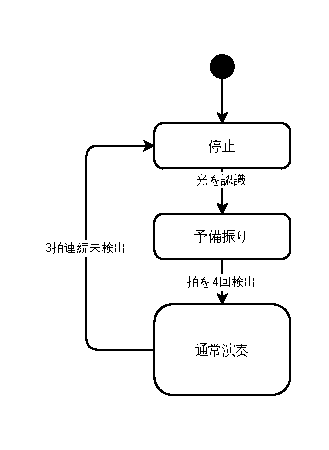
\includegraphics[width=0.8\linewidth]{figures/tantoB/B_state.pdf}
\caption{状態遷移図}
\label{fig:state_B}
\end{figure}

各状態は，センサーから取得した情報に基づいて以下の条件で遷移する．

\begin{itemize}

\item 停止状態 $\rightarrow$ 予備振り状態\\
累積拍検出回数（\texttt{detectCount}）が2以上であり，
かつ現在のループで拍が検出された場合に遷移する．

\item 予備振り状態 $\rightarrow$ 通常演奏状態\\
予備振り中の拍検出回数（\texttt{prebeatCount}）が4回に達した場合に遷移する
（\texttt{PREBEAT\_THRESH = 4}）．

\item 通常演奏状態 $\rightarrow$ 停止状態\\
最後の拍検出から推定拍間隔の3倍以上の時間が経過した場合に遷移する
（\texttt{MISSED\_BEAT\_THRESH = 3}）．

\end{itemize}

% ===================== 担当C =====================
\section{担当C — 楽譜・演奏制御}

\subsection{機能一覧}
担当Cでは，以下の2点を担当する．
\begin{enumerate}
  \renewcommand{\labelenumi}{(\arabic{enumi})}
  
\item \textbf{楽譜データの作成}

\item \textbf{Arduino-Processing間の通信システムの設計・実装}

\end{enumerate}

各楽器の演奏開始タイミングは，親機Processingから送信される輝度キューによって決定される．発表当日にProcessingの楽器指定ボタンから順番に入力することで各子機へスタートキューが送られる．演奏予定順序を表\ref{offset01}に示す．なお，最終的な順序は試聴によって調整を行う．
\begin{table}[H]
  \centering
  \caption{演奏予定順序（親機から動的に指示）}
  \label{offset01}
  \begin{tabular}{|c|c|c|}
\hline
楽器 & 演奏開始 & パート \\\hline \hline
ハイハット・シンバル & 0小節目 & リズム１ \\ \hline
バス・スネア & 0小節目 & リズム２ \\ \hline
鉄琴 & 2小節目 & 主旋律１ \\ \hline
ピアノ & 4小節目 & 主旋律２ \\ \hline
トランペット & 6小節目 & 主旋律３ \\ \hline
  \end{tabular}  
\end{table}
\FloatBarrier

演奏テンポは表\ref{テンポ}の通りである．\\
\begin{table}[h]
  \centering
  \caption{演奏テンポ一覧表}
  \label{テンポ}
  \begin{tabular}{|c|c|}
\hline
区間 & テンポ  \\\hline \hline
開始〜14小節（一周目演奏終了） & 80bpm \\ \hline
15小節目（二周目演奏開始）以降 & 104bpm  \\ \hline


  \end{tabular}  
\end{table}
\FloatBarrier

演奏用Arduino-Processing 間の通信は有線接続によってシリアル通信を行う．ArduinoからProcessingへ送信する内容一覧は表\ref{serial}に記す．

\begin{table}[h]
  \centering
  \caption{シリアル通信パケット仕様}
  \label{serial}
  \begin{tabular}{|c|c|c|c|c|}
\hline
バイト & フィールド名& 内容& 型 & 範囲  \\\hline \hline
0&NOTE\_OFF&前の音の終了&uint8&true = 1，false = 0 \\ \hline
1 & NOTE & 音名インデックス & uint8 &   0〜127（255 = 休符）\\ \hline
2 & VEL & 音の強さ & uint8 &   0〜127\\ \hline
  \end{tabular}  
\end{table}
\FloatBarrier

\subsection{システム構成図}
担当Cのシステム構成図は図\ref{system}の通りである．


\begin{figure}[H]
    \centering
    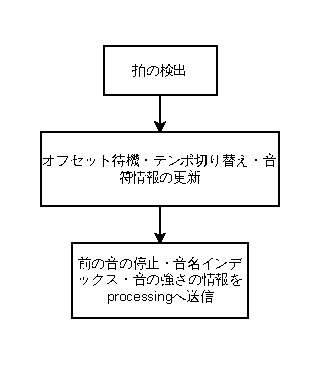
\includegraphics[,width=0.8\linewidth, keepaspectratio]{figures/tantoC/system.drawio.pdf}
    \caption{担当Cシステム構成図}
    \label{system}
\end{figure}



%\subsection{状態遷移図}

%\figspace[4]{状態遷移図を挿入}

% ===================== 担当D =====================
\section{担当D — 音響合成（Processing/Minim）}

\subsection{機能一覧}
本担当では，Arduino（担当C）から送信されるシリアル通信データを受信し，
Processing上で音響合成を行い，各楽器音をリアルタイムに出力する機能を実装する．

主な機能は以下の通りである．

\begin{itemize}

  \item シリアル通信受信機能 \\
  Arduinoから送信される4バイトパケット（NOTE\_OFF / NOTE / VEL / LONG）を受信し，
  前音の消音および新規発音イベントとして解釈する．
  ボーレートは115200\,bpsとする．

  \item 受信データパース機能 \\
  受信したバイト列を4バイト単位で解析し，
  NOTE\_OFF（\texttt{1}=前音停止 / \texttt{0}=継続），
  音名インデックス，ベロシティ，および音長（LONG）情報を抽出する．
  LONGは音価（\texttt{2}=2分音符 / \texttt{4}=4分音符 / \texttt{8}=8分音符）を表し，
  発音時にADSRの減衰（Decay）・余韻（Release）時間へ倍率として反映することで
  響き・余韻の長さを調整する（2分音符は長め，4分音符は標準，8分音符は短め）．
  なお，発音中の音を実際に停止するタイミングはLONGではなくNOTE\_OFF=1の受信で制御する．

  \item 音高変換機能 \\
  音名インデックス（C4=0, D4=1, E4=2, F4=3, G4=4, A4=5，休符=6）を
  MIDIノート番号へ変換し，
  $f = 440 \times 2^{(n-69)/12}$\,[Hz] により周波数を算出する．
  変換テーブルは担当Cと合意のうえ実装する．

  \item 音響合成機能 \\
  Minimライブラリを用い，Oscil・ADSR・フィルタ・BitCrusherを
  直列接続したUGenチェーンにより各楽器音をリアルタイムに生成する．

  \item 楽器音色生成機能 \\
  ハイハット・シンバル，バスドラム・スネア，鉄琴，ピアノ，トランペットの
  5パートそれぞれに対し，倍音比率・ADSRパラメータ・フィルタ設定を
  個別に定義し，識別可能な音色を実現する．

  \item 発音・消音制御機能 \\
  NOTE\_OFFフラグ=1のパケット受信時に前音のADSRリリースを開始し，
  続くNOTEバイトが休符（6）でなければ新規発音のアタックを開始する．
  新規発音時はLONG（音価）に応じてADSRの減衰・リリース時間に倍率を乗じ，
  響きの長さを音価に合わせて変化させる（消音の判断自体はLONGでは行わず，
  常にNOTE\_OFF=1の受信で制御する）．
  フェルマータ中は担当Cが次パケットの送信を保留するため，
  Processing側は特別な処理を行わずSustain状態を維持する．
  腕再開後に担当Cから次パケット（NOTE\_OFF=1）が送信された時点で
  リリースを開始し，新たな音の発音へ移行する．

  \item 多重発音機能 \\
  テンポ変化時などNOTE\_OFF=0のパケットを受信した場合，
  前音を強制消音せずに重ねて発音することで，
  音の途切れによる不自然さを回避する．

  \item 操作インターフェース機能 \\
  ハッカソン本番での迅速なセットアップを支援するため，
  シリアルポートの自動接続，マスターボリュームスライダー（0〜100\,\%），
  および受信した4バイトパケット（NOTE\_OFF / NOTE / VEL / LONG）の数値を
  リアルタイム表示するパネルをProcessing上に実装する．

  \item デバッグ・ログ出力機能 \\
  受信パケット（NOTE\_OFF / NOTE / VEL / LONG）のパース結果および発音・消音イベントの
  タイミングをシリアルモニタへ出力し，開発・動作確認を支援する．

\end{itemize}

\subsection{システム構成図}
本構成図では，担当D（Processing/Minim）の内部構成と，
上流の担当C（Arduino子機）および下流のスピーカー出力との接続関係を示す．

\begin{figure}[H]
    \centering
    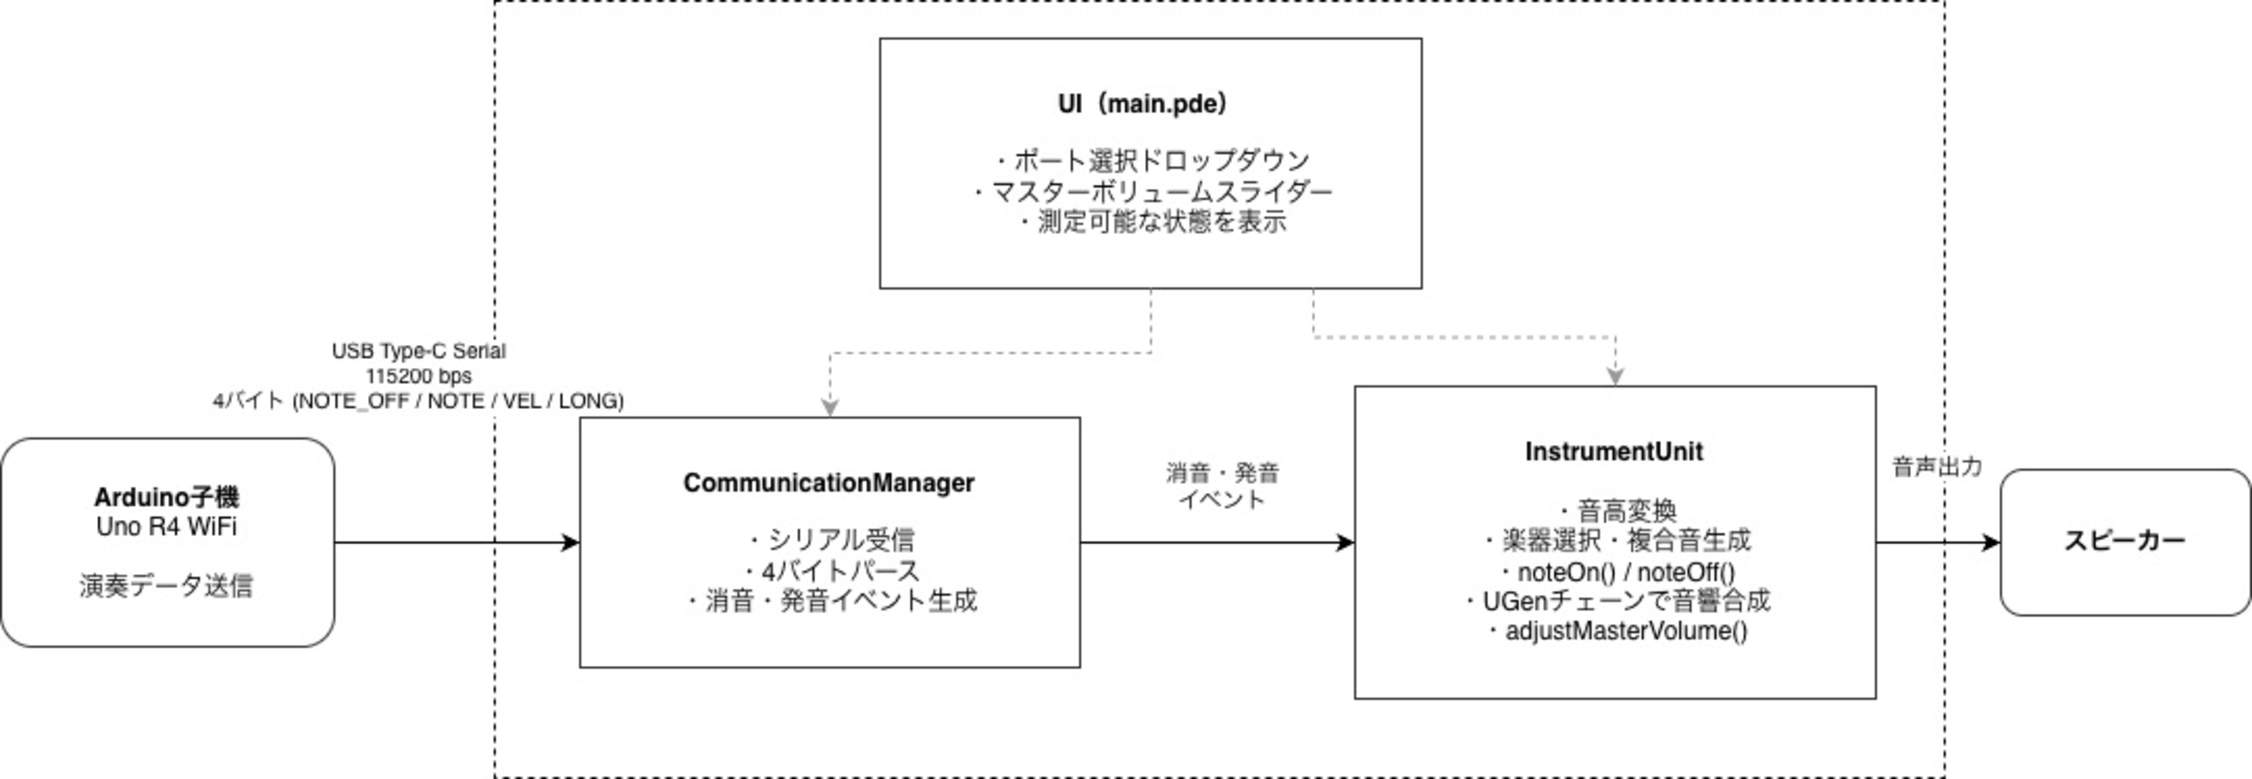
\includegraphics[width=0.8\linewidth]{figures/tantoD/system_diagram_D.pdf}
    \caption{担当Dシステム構成図}
    \label{fig:tantoD:system}
\end{figure}

図に示す通り，本システムは以下の3層で構成される．

\begin{description}
  \item[通信層 --- CommunicationManager]
  Arduino子機からUSB Type-C Serialを介して115200\,bpsで送信される
  4バイトパケット（NOTE\_OFF / NOTE / VEL / LONG）を受信・解析し，
  前音の消音および新規発音イベントとして音響層へ通知する．
  また，シリアルポートの自動接続およびログ出力を管理する．

  \item[音響合成層 --- InstrumentUnit]
  受信イベントに基づき，音高変換，楽器選択，波形生成，およびUGenチェーンによる
  音響合成処理を統括する．
  各楽器パートに対応するInstrumentUnitインスタンスを独立して保持し，
  多重発音にも対応する．

  \item[出力層 --- AudioOutput]
  Minimライブラリの\texttt{AudioOutput}を通じてスピーカーへ音響信号を送出する．
  マスターボリュームスライダーの値（0.0〜1.0）をデシベルに変換し，
  \texttt{out.setGain()}へ渡すことでアンサンブル全体の音量を調整可能とする．
\end{description}

各層間のデータフローを以下に示す．

\begin{center}
\texttt{Arduino子機} $\xrightarrow{\text{Serial 115200bps / 4B}}$
\texttt{CommunicationManager} $\xrightarrow{\text{発音・消音イベント}}$
\texttt{InstrumentUnit} $\xrightarrow{\text{UGenチェーン}}$
\texttt{AudioOutput} $\rightarrow$ \texttt{スピーカー}
\end{center}

なお，UGenチェーンの詳細（Oscil・ADSR・フィルタ・BitCrusherの接続構成）は
次節（音響合成チェーン）に示す．

\subsection{音響合成チェーン}
\label{sec:ugen}
受信したNOTE情報は，直ちに以下のUGenチェーンに渡され，
各楽器音がリアルタイムに合成・出力される．

\begin{center}
\texttt{Oscil（基音＋倍音）} $\rightarrow$
\texttt{ADSR} $\rightarrow$
\texttt{Filter（LowPassFS / HighPassFS）} $\rightarrow$
\texttt{BitCrusher} $\rightarrow$
\texttt{AudioOutput}
\end{center}

\begin{figure}[H]
    \centering
    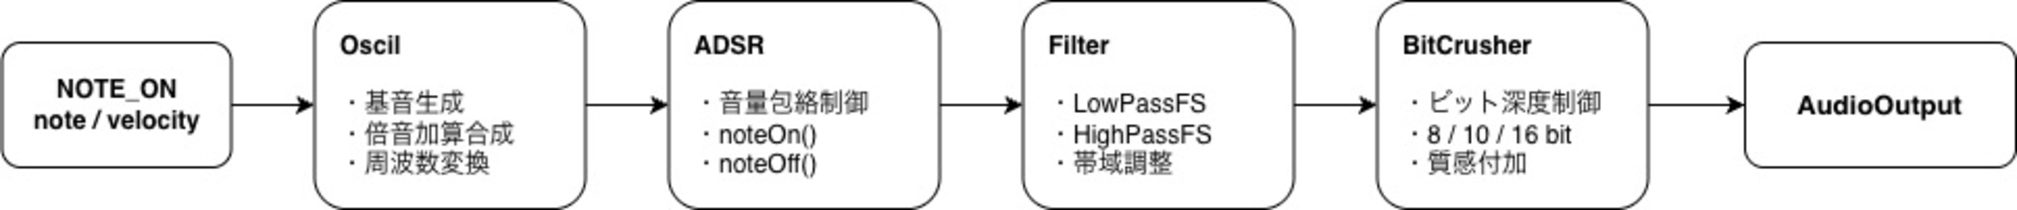
\includegraphics[width=0.8\linewidth]{figures/tantoD/ugen_chain_diagram.pdf}
    \caption{UGen合成チェーン図}
    \label{fig:tantoD:ugen}
\end{figure}

基音の生成から始まり，倍音の付加，ADSRによる音量エンベロープの適用，
フィルタによる帯域調整，BitCrusherによる質感付加を経て，
最終的なスピーカー出力となる．
各ユニットの詳細なパラメータ設定については詳細設計に示す．

なお本チェーンは有音程楽器（ピアノ・鉄琴・トランペット）およびバスドラムの標準形である．
実装上，ピアノはデジタル感を避けるためBitCrusherを省略し，
シンバルはOscilチェーンではなく事前生成したモーダル波形を\texttt{Sampler}経由で出力する．
また\texttt{HighPassFS}は現行実装では使用せず，全楽器\texttt{LowPass}である．

\subsection{操作インターフェース設計}
ハッカソン本番の現場における迅速なセットアップと，
開発・デバッグ時の動作確認を目的として，
Processing上に以下のコントロールパネルを実装する．

\subsubsection{シリアルポート接続（自動接続）}
各PCにおけるArduinoの認識状況（ポート名）が異なることを想定し，
起動時に\texttt{usbmodem}／\texttt{usbserial}を含むポートを自動的に探索して接続する．
該当がなければ先頭のポートに接続し，接続できない場合はキーボード入力による動作確認のみ可能とする．
接続状態（接続済み／未接続）は画面に表示し，現場での確認を支援する．

\subsubsection{マスターボリューム・コントロール}
5台のPCから出力される音量を合奏形式で調整するため，
0〜100\,\%の範囲で操作可能なマスターボリュームスライダーを設ける．
各PCのOS音量設定に依存することなく，
アンサンブルの聴感上のバランスをリハーサル中に即座に最適化できる．

\subsubsection{受信データモニタ}
開発・デバッグ時の動作確認を目的として，
受信した4バイトパケット（NOTE\_OFF / NOTE / VEL / LONG）の数値と，
シリアル接続状態（接続済み／未接続）をリアルタイムに表示するパネルを実装する．

設計当初はIDLE / PLAYING / FERMATA等のシステム状態表示を検討したが，
確定仕様の4バイトパケットには担当BのSTATE情報が含まれず，
Processing側で状態を確実に判定できないため，受信値そのもの（および接続状態）の表示とした．
なお，担当Cとの合意により4バイトパケットにSTATE情報（1バイト）を追加すれば，
状態表示へ拡張することが可能である．

\subsection{状態遷移図}
本システムはイベント駆動型であり，
Arduinoからのパケット受信をトリガとして動作する．
明示的な状態変数はもたず，発音中のボイス（\texttt{activeVoices}）の有無に応じて，
概念的にIDLE／PLAYINGの2状態として表せる．

\begin{figure}[H]
    \centering
    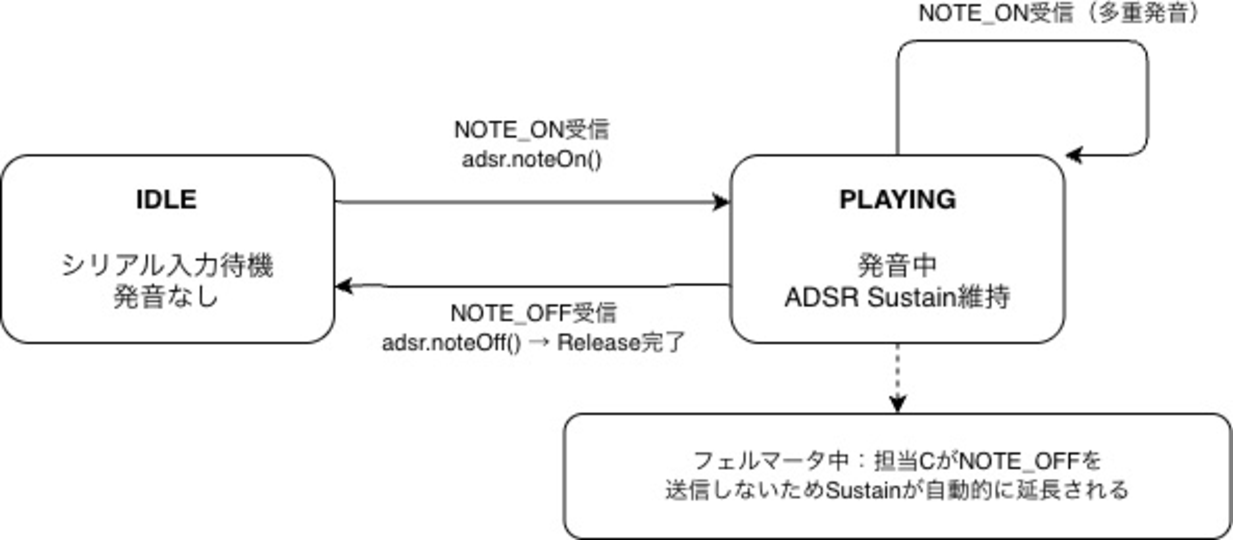
\includegraphics[width=0.8\linewidth]{figures/tantoD/state_transition_diagram_D.pdf}
    \caption{担当D状態遷移図}
    \label{fig:tantoD:state}
\end{figure}

\begin{description}
  \item[IDLE]
  発音中のボイスが存在しない状態（無音・入力待機）．
  発音パケット（NOTE $\neq$ 6）の受信により新規ボイスが生成され，PLAYINGへ移る．

  \item[PLAYING]
  1つ以上のボイスが発音中の状態．各ボイスはADSRに従って音を維持する．
  NOTE\_OFF=1を含む次パケットの受信で発音中のボイスがReleaseへ移行し，
  すべてのボイスが消えるとIDLEへ復帰する．
  フェルマータ中は担当Cが次パケットの送信を保留するため，Sustainが自動的に延長され，
  腕再開後に担当Cから次パケットが送信された時点でReleaseを開始する．
\end{description}

なお，各パートは専用スケッチとして1台のPCで独立に動作する（パート間は別プログラム）．
各パート内では1つのInstrumentUnitが複数のボイスを保持し，
各ボイスが独立したADSRライフサイクルをもつことで多重発音を実現する．

% =============================================================
\chapter{システムの詳細設計}

設計書は作成する成果物によって変化します．適宜修正して利用してください．

% ===================== 担当A =====================
\section{担当A — 指揮者人形・センサ機構}

\subsection{部品一覧}
本システムの構築にあたって，使用を想定している主要部品を以下の表\ref{tantoA:parts}に示す．

\begin{table}[h]
    \caption{部品一覧}
    \resizebox{\textwidth}{!}{%
    \begin{tabular}{lll}
        \hline
        部品名 & 型番・仕様 & 備考\\\hline
        マイクロコントローラ & Arduino Uno R4 WiFi & システム全体の制御を担当\\
        サーボモータ & SG92R & 負荷に応じて金属製ギアのものに変更\\
        反射板（腕） & プラスチックなど & 軽量かつ赤外線を反射しやすい素材を選定\\
        指揮用LED & 高輝度単色LED（赤または白） & 子機センサが検知しやすいものを選定\\
        状態表示用LCD & SSCI-014076 & BPMや状態を表示 \\\hline
    \end{tabular}
    }
    \label{tantoA:parts}
\end{table}

\subsection{ハードウェア設計}
\subsubsection{ユニット構成}
本ユニットにおける具体的な設計案を以下の図\ref{tantoA:conductor}に示す．

\begin{figure}[h]
    \centering
    
\includegraphics[width=10cm]{figures/blueprint.pdf}
    \caption{指揮者人形ユニットの設計図}
    \label{tantoA:conductor}
\end{figure}

本ユニットは，制御・処理を担うマイクロコントローラ（Arduino Uno R4 WiFi），腕の物理動作を行うサーボモータ，
拍タイミングを光で提示する指揮用LED，演奏状態を表示するLCDディスプレイで構成される．\par

なお，赤外線測距センサおよびフォトトランジスタは本ユニットには搭載しない．
これらは各楽器ユニット（子機）側に搭載され，指揮者人形ユニット（親機）の腕（反射板）の位置変化および指揮用LEDの点灯を観測することで，
通信に依存せず自律的に拍を同期する役割を担う．

\subsubsection{ピン接続}
Arduino Uno R4 WiFiと各デバイスのピン接続を以下の表\ref{tantoA:pins}に示す．

\begin{table}[h]
\caption{ピン接続一覧}
\begin{tabular}{lll}
    \hline
    Arduinoピン & 接続先デバイス & 信号種別 \\\hline
    D9（PWM） & サーボモータ & PWM出力 \\
    D7 & 指揮用LEDアノード（330Ω経由） & デジタル出力 \\
    SDA & LCD（SSCI-014076） & I$^2$C データ \\
    SCL & LCD（SSCI-014076） & I$^2$C クロック \\
    USB Type-C & PC（Processing） & シリアル通信（115200bps） \\
    \hline
\end{tabular}
\label{tantoA:pins}
\end{table}

\subsubsection{回路設計}
本ユニットにおける回路接続図を以下の図\ref{tantoA:circuit}に示す．

\begin{figure}[h]
    \centering
    
\includegraphics[width=10cm]{figures/Unit_circuit.pdf}
    \caption{回路接続図}
    \label{tantoA:circuit}
\end{figure}

\subsection{ソフトウェア設計}
\subsubsection{概要}
本ユニットのソフトウェアは，Arduino Uno R4 WiFi上で動作するファームウェアと，PC乗で動作する制御アプリケーション（Processing）の2つで構成される．\par

ファームウェアは，演奏の状態管理・サーボモータの制御・LED点灯・LCD表示・シリアル通信受信を担う．
状態管理には「待機」「予備拍」「演奏中」「フェルマータ」「演奏停止」の5つの状態を定義し，PCからのコマンド受信をトリガとして状態を遷移させる．
拍のタイミング生成にはFspTimerによる割り込みを用い，メインループに依存しないマイクロ秒単位の精度でサーボモータとLEDを同期制御する．\par

制御アプリケーション（Processing）は，ユーザのボタン操作に応じてSTART・STOP・FERMATAの各コマンドをシリアル通信（115200bps）経由でArduinoへ送信する役割を担う．

\subsubsection{シリアル通信プロトコル}
PCからArduinoへ送信するコマンドの仕様を表\ref{tantoA:protocol}に示す．

\begin{table}[H]
\caption{シリアル通信コマンド仕様}
\centering
\begin{tabular}{lll}
    \hline
    コマンド文字列 & 意味 & 遷移先状態 \\\hline
    \texttt{START} & 演奏開始 & 予備拍 → 演奏中 \\
    \texttt{STOP}  & 演奏停止 & 停止動作 → 待機 \\
    \texttt{FERMATA} & フェルマータ開始 & フェルマータ \\
    \hline
\end{tabular}
\label{tantoA:protocol}
\end{table}

\subsubsection{関数設計}
Arduinoのファームウェアおよび制御アプリケーション（Processing）それぞれの関数一覧を以下の表\ref{tantoA:func_arduino}，表\ref{tantoA:func_processing}に示す．

\begin{table}[H]
\caption{Arduino側 関数一覧}
\centering
\resizebox{\textwidth}{!}{%
\begin{tabular}{llll}
    \hline
    関数名 & 引数 & 戻り値 & 役割 \\\hline
    \texttt{setup()} & なし & なし & 各デバイスの初期化，タイマ割り込みの設定 \\
    \texttt{loop()} & なし & なし & シリアル受信の監視，状態に応じた処理の呼び出し \\
    \texttt{onBeatTimer()} & なし & なし & タイマ割り込み：サーボ角度更新・LED点灯を同期実行 \\
    \texttt{updateServo()} & なし & なし & 現在の状態・拍位相に基づきサーボ角度を更新 \\
    \texttt{updateLED()} & なし & なし & 拍の最前点でLEDを短時間点灯させる \\
    \texttt{receiveCommand()} & なし & なし & シリアルバッファを読み取りコマンド文字列を返す \\
    \texttt{changeState(State s)} & 遷移先状態 \texttt{s} & なし & 状態変数を更新し，遷移時の初期化処理を行う \\
    \texttt{updateLCD()} & なし & なし & 現在の状態・BPMをLCDに表示する \\
    \hline
\end{tabular}
}
\label{tantoA:func_arduino}
\end{table}

\paragraph{制御アプリケーション（Processing）}

\begin{table}[H]
\caption{Processing側 関数一覧}
\centering
\resizebox{\textwidth}{!}{%
\begin{tabular}{llll}
    \hline
    関数名 & 引数 & 戻り値 & 役割 \\\hline
    \texttt{setup()} & なし & なし & ウィンドウ・シリアルポートの初期化，UIボタンの配置 \\
    \texttt{draw()} & なし & なし & UIの再描画（ボタン状態・接続状態の表示更新） \\
    \texttt{mousePressed()} & なし & なし & クリック座標からボタンを判定し対応コマンドを送信 \\
    \texttt{sendCommand(String cmd)} & 送信コマンド文字列 \texttt{cmd} & なし & シリアルポート経由でArduinoへコマンドを送信 \\
    \texttt{drawButton(String label, int x, int y)} & ラベル，X座標，Y座標 & なし & 指定位置にボタンを描画する \\
    \hline
\end{tabular}
}
\label{tantoA:func_processing}
\end{table}

\subsection{処理フローの設計}
メインループ処理およびタイマ割り込みの処理フロー図を以下の図\ref{tantoA:mainloop}，図\ref{tantoA:timer}に示す．

\begin{figure}[H]
    \centering
    
\includegraphics[width=8cm]{figures/mainloop.pdf}
    \caption{メインループ処理の処理フロー図}
    \label{tantoA:mainloop}
\end{figure}

\begin{figure}[H]
    \centering
    
\includegraphics[width=8cm]{figures/timer.pdf}
    \caption{タイマ割り込みの処理フロー図}
    \label{tantoA:timer}
\end{figure}

\subsection{テストの設計}
本ユニットの動作検証におけるテスト方針、および具体的なテスト項目について記述する。

\subsubsection{テスト方針}
本ユニットはシステム全体の親機として機能し、正確なテンポ維持とPCからのコマンドに応じた柔軟な状態遷移が求められる。
そのため、テストは「ハードウェア単体テスト」「ソフトウェア機能テスト」「システム統合テスト」の3段階に分けて実施し、段階的に信頼性を確保する。

\subsubsection{テスト項目一覧}
具体的なテスト項目、検証内容、およびテストデータを表\ref{tantoA:test_cases}に示す。

\begin{table}[H]
\caption{テスト項目一覧}
\centering
\resizebox{\textwidth}{!}{%
\begin{tabular}{llll}
    \hline
    カテゴリ & テスト項目名 & 検証内容 & テストデータ・条件 \\\hline
    ハードウェア単体 & サーボモータ動作検証 & 指定した角度へ正確に追従し、腕（反射板）の負荷で脱調しないか & 動作角度：0\textdegree〜$\pm$30\textdegree \\
    & 指揮用LED視認性検証 & LEDが十分な光量で点灯し、子機側センサで検知可能か & 点灯時間：最前点での短時間パルス点灯 \\
    & LCD表示検証 & 動作状態やBPMが文字化けや遅延なく正しく表示されるか & 各状態の文字列、BPM：60〜140 \\\hline
    ソフトウェア機能 & シリアル通信・状態遷移 & 各コマンド受信により、定義された5つの状態へ正しく遷移するか & \texttt{START}, \texttt{STOP}, \texttt{FERMATA}、および予備拍・待機状態 \\
    & タイマ割り込み精度 & FspTimerによる割り込みがメインループに依存せず正確に作動するか & 各種BPM設定時における割り込み周期の計測 \\\hline
    システム統合 & E2Eフロー検証 & ProcessingのUI操作からコマンド送信、物理動作まで一連のフローが機能するか & 各種ボタンのクリック操作（START $\rightarrow$ FERMATA $\rightarrow$ STOPなど） \\
    & BPM境界値検証 & 高速・低速動作時にサーボの追従遅れやタイマの処理落ちがないか & 最小設定BPM、最大設定BPM \\
    \hline
\end{tabular}
}
\label{tantoA:test_cases}
\end{table}

\section{担当B — センサ処理・状態機械}

担当 B は，子機 Arduino における指揮者人形の観測・テンポ推定・状態管理を担う．
センサ構成はフォトトランジスタ（デジタル入力）とカラーセンサ（I2C）の 2 種類であり，
両センサの情報を組み合わせてテンポ推定と演奏開始判定を行い，発音タイミングを決定する．

\subsection{部品一覧}

\begin{table}[H]
\centering
\caption{使用部品一覧}
\label{tab:parts_B}
\begin{tabular}{p{4cm}p{5cm}p{2.5cm}p{3cm}}
\hline
\textbf{部品名} & \textbf{型番} & \textbf{ピン} & \textbf{用途} \\
\hline
フォトトランジスタ（$\times$5） & NJL7502L (560nm) & D4 & 拍タイミング検出（デジタル入力） \\
\hline
カラーセンサ（$\times$5） & AE\_S13683\_LED & I2C (SDA/SCL) & 演奏開始キュー（色）判別 \\
\hline
Arduino（子機） & Arduino Uno R4 WiFi & — & センサ処理・テンポ推定・状態管理 \\
\hline
\end{tabular}
\end{table}

\subsection{ハードウェア設計}

フォトトランジスタ（NJL7502L）はデジタルピン \texttt{D4} に接続し，
\texttt{HIGH} / \texttt{LOW} の二値で受光量を取得する．
カラーセンサ（AE\_S13683\_LED）はI2Cバス（SDA/SCL）に接続し，
ワンショット測定モードで RGB 値を取得する．

Arduinoと各デバイスのピン接続を表\ref{tab:pins_B}に示す．

\begin{table}[H]
\centering
\caption{ピン接続一覧}
\label{tab:pins_B}
\begin{tabular}{p{2.5cm}p{4cm}p{2.5cm}p{4cm}}
\hline
\textbf{Arduinoピン} & \textbf{接続先デバイス} & \textbf{信号種別} & \textbf{用途} \\
\hline
D4 (\texttt{PHOTO\_PIN}) & フォトトランジスタ & デジタル入力 & 拍タイミング検出 \\
\hline
SDA / SCL                & カラーセンサ（AE\_S13683\_LED） & I2C & 演奏開始キュー色判別 \\
\hline
\end{tabular}
\end{table}

図\ref{fig:circuit_B} に回路図を示す．

\begin{figure}[H]
\centering
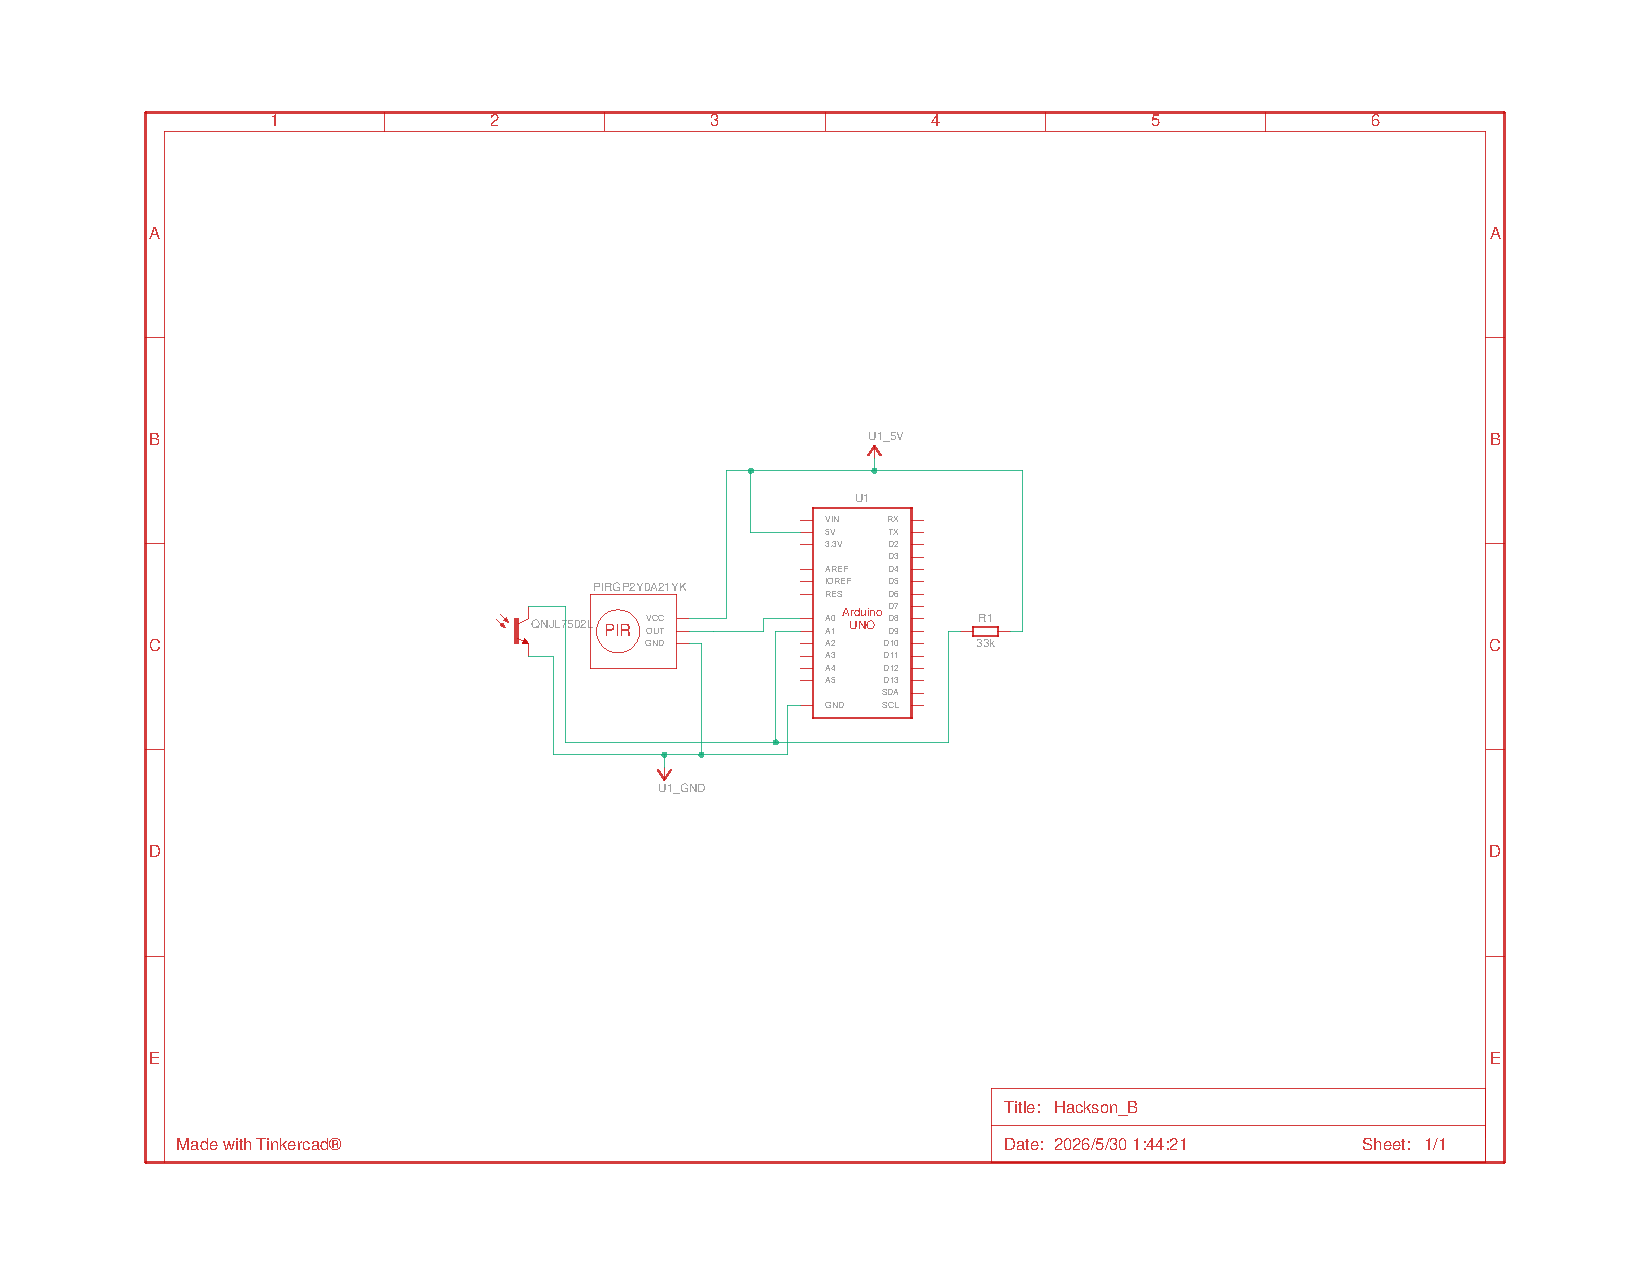
\includegraphics[width=0.8\linewidth]{figures/tantoB/Kairo_B.pdf}
\caption{回路図}
\label{fig:circuit_B}
\end{figure}

\subsection{ソフトウェア設計}

\subsubsection{ファイル構成}

\begin{table}[H]
\centering
\caption{ファイル構成}
\begin{tabular}{p{5cm}p{8cm}}
\hline
\textbf{ファイル名} & \textbf{内容} \\
\hline
\texttt{hackson\_main.ino} & BとCの共通部分．\texttt{setup()} および \texttt{loop()} のエントリポイント，共有変数の宣言，カラーセンサの初期化を含む． \\
\hline
\texttt{B.ino} & 担当Bの独立部分．フォトトランジスタポーリング・カラーセンサ判別・テンポ推定・状態機械の実装． \\
\hline
\texttt{C.ino} & 担当Cの独立部分．発音タイミング制御・シリアル送信の実装． \\
\hline
\texttt{AE\_S13683\_LED.h / .cpp} & カラーセンサ（AE\_S13683\_LED）のドライバライブラリ． \\
\hline
\end{tabular}
\end{table}

\subsubsection{オブジェクト設計（主要変数）}

\begin{lstlisting}[caption=担当 B 主要変数（B.ino / hackson\_main.ino）]
// ---- hackson_main.ino で宣言（担当Cと共有） ----
unsigned long          nextBeatTime    = 0;    // 次の拍予測絶対時刻 [ms]
volatile unsigned long currentBeatTime = 0;    // 現在の拍検出時刻 [ms]
volatile unsigned long lastBeatTime    = 0;    // 最後の拍検出時刻 [ms]
bool                   beatUpdated     = false; // nextBeatTime 更新フラグ
bool                   isPlaying       = false; // 演奏開始フラグ
enum                   State           {IDLE, PREBEAT, PLAYING};
State                  state           = IDLE;  // 現在の状態

// ---- B.ino で宣言（担当B専用） ----
// カラーセンサ
const char* colorName       = "Unknown"; // 検出した色名
const char* PLAY_COLOR_NAME = "Red";     // 自楽器の演奏開始色（楽器ごとに変更する）

// フォトトランジスタ
volatile bool beatDetected = false; // 拍検出フラグ（1ループで1回処理後リセット）
int           detectCount  = 0;     // 累積拍検出回数
bool          high         = false; // 現在のデジタル読み取り値
bool          stateHigh    = false; // 立ち上がりエッジ検出用フラグ

// EMA テンポ推定
float         estimatedBeatInterval = 1000.0f; // 推定拍間隔 [ms]
float         emaAlpha              = 0.2f;     // EMA 係数
unsigned long previousBeatTime      = 0;        // 前回拍検出時刻 [ms]
const float   TEMPO_CHANGE_THRESH   = 10.0f;   // テンポ急変検出閾値 [%]
float         previousNextBeatTime  = 0;        // 前回予測次拍時刻

// 状態機械
int       prebeatCount       = 0; // 予備振り中の拍検出回数
const int PREBEAT_THRESH     = 4; // 予備振り必要回数
const int MISSED_BEAT_THRESH = 3; // 演奏停止判定の未検出拍数倍率
\end{lstlisting}

\subsubsection{担当Cとの共有変数}

担当 B と担当 C は同一の Arduino 上で動作するため，以下のグローバル変数を共有することで連携する．
担当 B が書き込み，担当 C が読み取る変数を以下に示す．

\begin{table}[H]
\centering
\caption{担当 C との共有変数一覧}
\begin{tabular}{p{3.5cm}p{2.5cm}p{4cm}p{4cm}}
\hline
\textbf{変数名} & \textbf{型} & \textbf{担当Bの役割} & \textbf{担当Cの使い方} \\
\hline
\texttt{nextBeatTime} & \texttt{unsigned long} &
次の拍の予測絶対時刻を書き込む & 信号送信タイミングの基準として読む \\
\hline
\texttt{beatUpdated} & \texttt{bool} &
\texttt{nextBeatTime} が更新されたら \texttt{true} にする &
\texttt{true} を検知して処理後 \texttt{false} に戻す \\
\hline
\texttt{state} & \texttt{State} &
現在の演奏状態を書き込む &
IDLE 判定などに使う \\
\hline
\texttt{isPlaying} & \texttt{bool} &
カラーキュー一致時に \texttt{true} にする &
演奏開始のトリガーとして使う \\
\hline
\texttt{currentBeatTime} & \texttt{unsigned long} &
現在の拍検出時刻を書き込む &
\texttt{sendTime} 補正計算に使う \\
\hline
\end{tabular}
\end{table}

なお，\texttt{beatUpdated} を \texttt{false} にリセットする責任は担当 C 側にある．

\subsubsection{関数設計}

\begin{table}[H]
\centering
\footnotesize
\setlength{\tabcolsep}{3pt}
\renewcommand{\arraystretch}{1.1}
\caption{担当 B 主要関数一覧}
\label{tab:func_B}
\resizebox{\textwidth}{!}{%
\begin{tabular}{p{3.8cm}p{3.2cm}p{3.2cm}p{5.2cm}}
\hline
\textbf{関数名} & \textbf{入力} & \textbf{出力} & \textbf{役割} \\
\hline
\texttt{void photoISR()} &
PHOTO\_PIN（D4） &
high, stateHigh,
beatDetected,
currentBeatTime,
lastBeatTime &
デジタルピンをポーリングし，LOW→HIGHの立ち上がりエッジで拍を検出する．
前回検出から200\,ms以内は無視する（チャタリング防止）． \\
\hline
\texttt{const char*} \texttt{detectColor} \texttt{(float r,} \texttt{float g,} \texttt{float b)} &
RGB浮動小数点値 &
色名文字列（戻り値） &
入力RGB値を正規化し，7種の参照色（Red / Green / Blue / Yellow / Cyan / Magenta / White）とのコサイン類似度を計算して最も類似した色名を返す． \\
\hline
\texttt{void readColor()} &
カラーセンサ（I2C） &
colorName &
カラーセンサからワンショット測定でRGBを取得し，detectColor()で色名に変換してcolorNameを更新する．拍検出時のみ呼び出す． \\
\hline
\texttt{void updateTempoByPhoto()} &
currentBeatTime,
previousBeatTime,
estimatedBeatInterval,
state &
estimatedBeatInterval,
previousBeatTime,
nextBeatTime,
previousNextBeatTime &
拍間隔をEMAでテンポ推定する．
PLAYING状態かつ誤差率がTEMPO\_CHANGE\_THRESH（10\%）を超えた場合はEMAをバイパスして実測値を直接採用する．PREBEAT状態では常にEMAを適用する． \\
\hline
\texttt{void updateState()} &
beatDetected,
detectCount,
prebeatCount,
lastBeatTime,
estimatedBeatInterval &
state,
isPlaying,
prebeatCount &
IDLE / PREBEAT / PLAYINGの3状態を管理する．
各状態の遷移条件を判定し，stateを更新する． \\
\hline
\texttt{void B\_loop()} &
— &
— &
担当Bのメインループ処理．
photoISR()呼び出し→拍検出時のカラー判別・テンポ更新→状態遷移の順に実行する． \\
\hline
\end{tabular}
}
\end{table}

\subsection{処理フローの設計}

\begin{figure}[H]
  \centering
  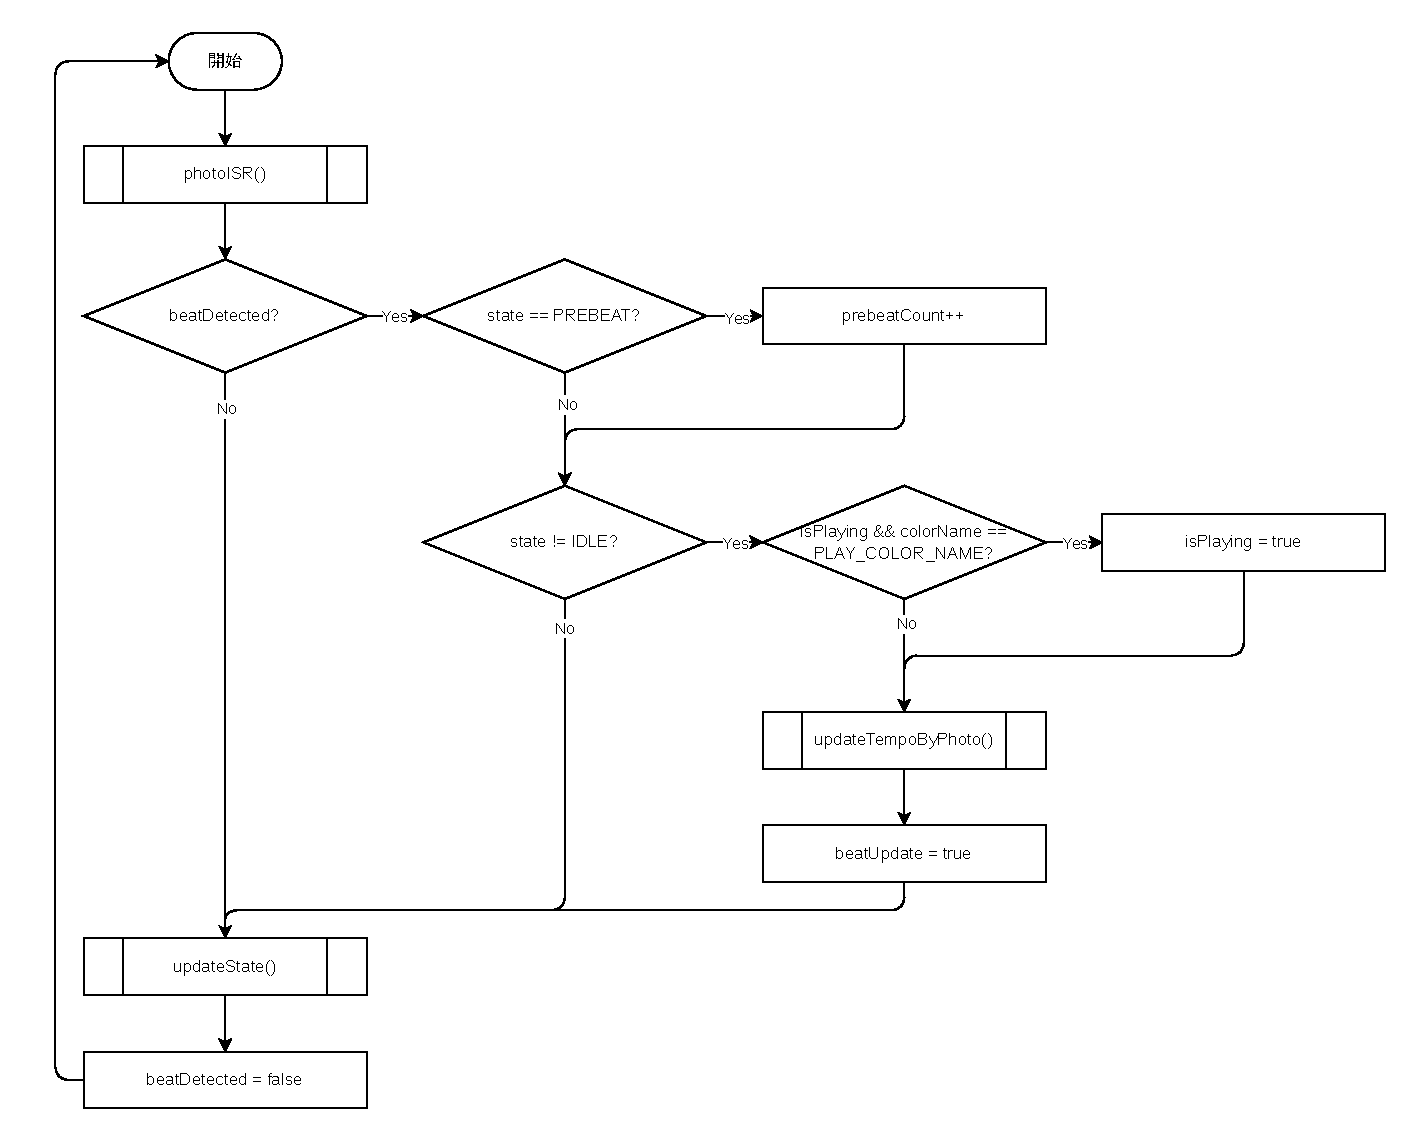
\includegraphics[width=0.8\linewidth]{figures/tantoB/flowchart_B_loop.pdf}
  \caption{B\_loop}
\end{figure}

\begin{figure}[H]
  \centering
  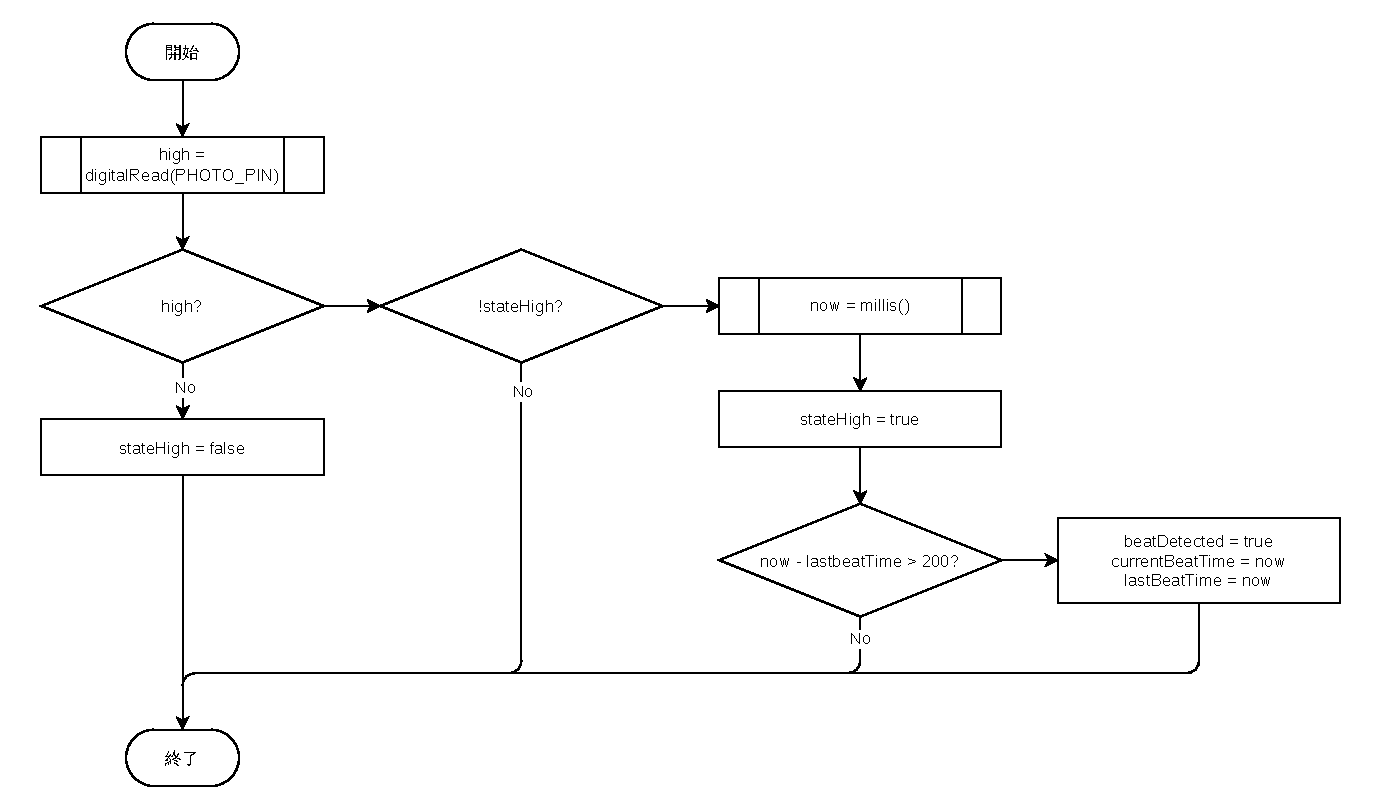
\includegraphics[width=0.8\linewidth]{figures/tantoB/flowchart_photoISR.pdf}
  \caption{photoISR}
\end{figure}

\begin{figure}[H]
  \centering
  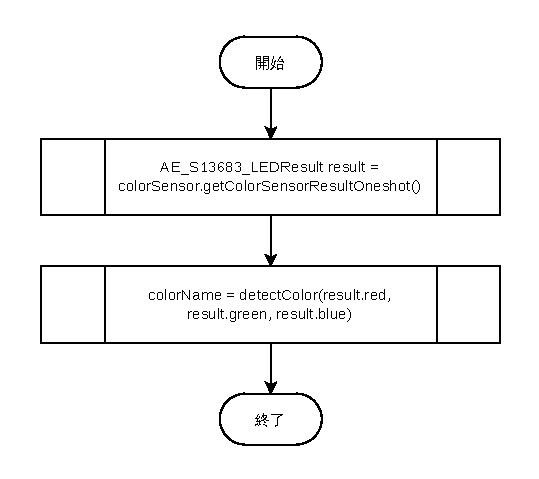
\includegraphics[width=0.8\linewidth]{figures/tantoB/flowchart_readColor.pdf}
  \caption{readColor}
\end{figure}

\begin{figure}[H]
  \centering
  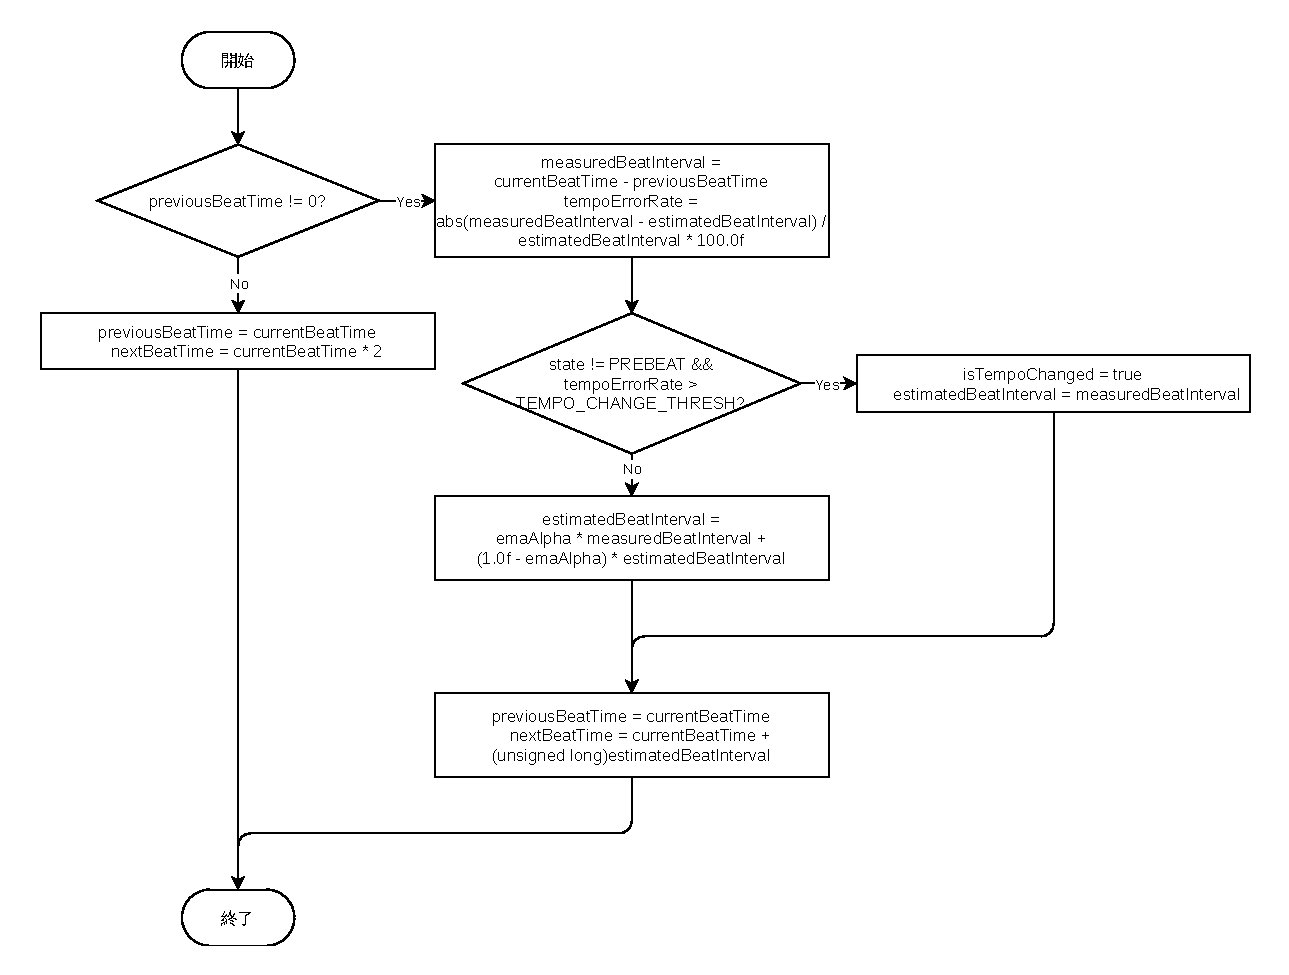
\includegraphics[width=0.8\linewidth]{figures/tantoB/flowchart_updateTempoByPhoto.pdf}
  \caption{updateTempoByPhoto}
\end{figure}

\begin{figure}[H]
  \centering
  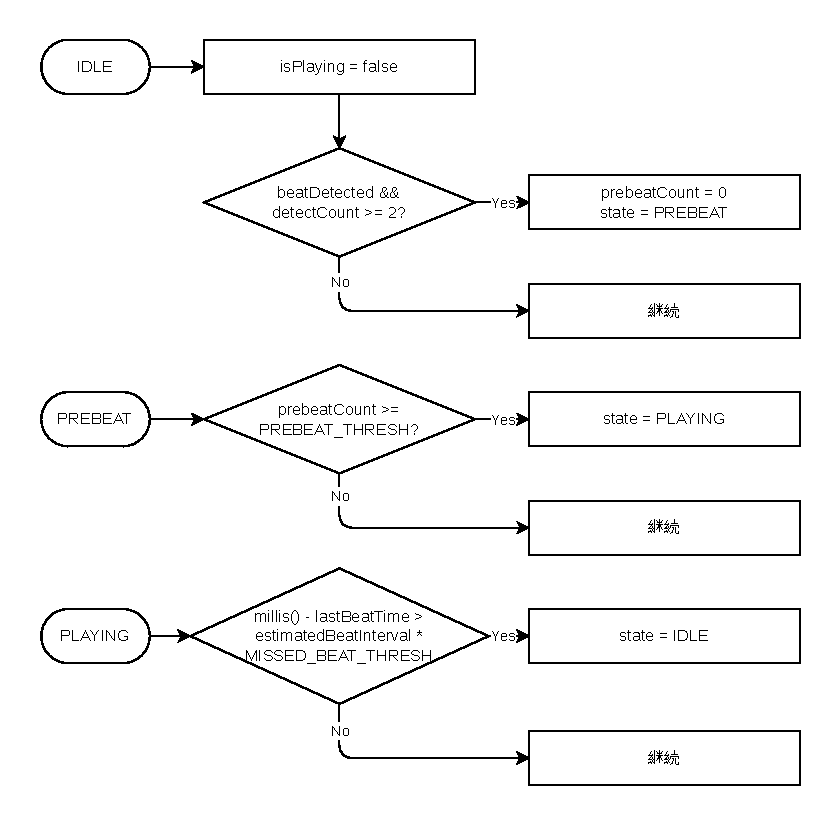
\includegraphics[width=0.8\linewidth]{figures/tantoB/flowchart_updateState.pdf}
  \caption{updateState}
\end{figure}

\subsection{テストの設計}

担当Bが実施すべきテストの一覧を表\ref{tab:test_B}に示す．

\begin{table}[H]
\centering
\caption{テスト一覧}
\label{tab:test_B}
\begin{tabular}{p{3.5cm}p{5cm}p{4cm}}
\hline
\textbf{テスト名} & \textbf{内容} & \textbf{合格基準} \\
\hline
拍検出精度確認 &
指揮者LEDをメトロノームに合わせて点滅させ，
\texttt{photoISR()}が正しく拍を検出するか確認する．
また200\,ms以内の再検知が無視されることを確認する． &
検出成功率95\%以上，誤検出なし \\
\hline
カラーキュー判別確認 &
各楽器に対応する色（Red/Green/Blue/Yellow/White）を親機LEDで発光させ，
\texttt{detectColor()}が正しい色名を返すか確認する．
またシリアルモニタで \texttt{colorName} を観察する． &
5色全て正しく判別，誤判別なし \\
\hline
EMAテンポ推定精度確認 &
メトロノーム（80\,bpm，104\,bpm）に合わせて指揮動作を行い，
シリアルモニタで \texttt{estimatedBeatInterval} から換算したBPMを計測する． &
BPM誤差 $\pm$5\,bpm以内 \\
\hline
状態機械遷移確認 &
3状態の遷移シーケンスをシリアルモニタでトレースする．
IDLE→PREBEAT→PLAYINGおよびPLAYING→IDLEを確認する． &
設計通りの遷移のみ発生，無効遷移なし \\
\hline
演奏開始フラグ連携確認 &
\texttt{isPlaying}フラグが立った直後に担当Cが演奏パケットを送信するか確認する． &
色検出から1拍以内に演奏開始 \\
\hline
B-C間遅延測定（結合） &
拍検出タイムスタンプとNOTE\_ON送信タイムスタンプの差をシリアルで計測する． &
遅延 $\leq$50\,ms \\
\hline
A-B間テンポ追従確認（結合） &
人形BPMを80→104に変化させ，担当BのEMAが追従するか確認する． &
3小節以内に新テンポに収束 \\
\hline
\end{tabular}
\end{table}

% ===================== 担当C =====================
\section{担当C — 楽譜・演奏制御}

\subsection{部品一覧}
担当Cで必要となる器具と環境について表\ref{need}に記す．

\begin{table}[H]
  \centering
  \caption{事前に揃えるべき器具・環境}
  \label{need}
  \begin{tabular}{|c|c|c|}
\hline
品目 & 数量 & 用途 \\\hline \hline
Arduino Uno R4 Wifi（子機用） & 5 & 楽器ユニット各1台 \\ \hline
USB Type-Cケーブル & 5 & 各子機とPC缶のSerial通信 \\ \hline
シリアル通信テスト環境（Arduino IDE シリアルモニタ）& - & C1テスト（B-C間遅延測定） \\ \hline
  \end{tabular}  
\end{table}



%\subsection{ハードウェア設計}
%（ここに記載）

\subsection{ソフトウェア設計}
%\subsubsection{ファイル構成}
%（ここに記載）

\subsubsection{楽譜データ構造}
本システムで実装する楽譜データ構造は音名インデックス，音の強さ，拍数の3要素を持つ二次元配列として定義する．音名インデックスの定義一覧は以下の通りである．\\

音名インデックス：$C4=0，D4=1，E4=2，F4=3，G4=4，A4=5（休符：6）$\\

定義例はソースコード\ref{index}の通りである．各パートの最後は休符を設定する．

\begin{figure}[H]
\renewcommand{\lstlistingname}{ソースコード}
    \begin{lstlisting}[
        language=C++,
        caption={楽譜配列（カエルの歌）},
        label=index,
        escapechar=@,
        frame=single,
        basicstyle=\ttfamily\small,
        breaklines=true
    ]
const uint8_t score[][3] = {
   {0, 100, 1},   //ド
   {1, 100, 1},   //レ
   {2, 100, 1},   //ミ
   {3, 100, 1},   //ファ
   // ... 以下省略（前章節分を定義）
   };
   
   const int SCORE_LEN = sizeof ( score ) / sizeof ( score [0] ) ;

   \end{lstlisting}
\end{figure}

\subsubsection{テンポ管理・演奏制御用の定数}
各楽器の演奏開始は親機からの輝度キューによって決定される．子機は自機IDに対応する輝度レベルを検出した時点でスタートフラグを立て，次の拍タイミングで演奏を開始する．演奏予定順序を参考として表\ref{offset02}に示す．
\begin{table}[H]
  \centering
  \caption{演奏予定順序（親機から動的に指示）}
  \label{offset02}
  \begin{tabular}{|c|c|c|}
\hline
楽器 & 演奏開始 & パート \\\hline \hline
ハイハット・シンバル & 0小節目 & リズム１ \\ \hline
バス・スネア & 0小節目 & リズム２ \\ \hline
鉄琴 & 2小節目 & 主旋律１ \\ \hline
ピアノ & 4小節目 & 主旋律２ \\ \hline
トランペット & 6小節目 & 主旋律３ \\ \hline
  \end{tabular}  
\end{table}
\FloatBarrier

小節管理に使用する定数はソースコード\ref{beat}の通りである．
\begin{figure}[H]
\renewcommand{\lstlistingname}{ソースコード}
    \begin{lstlisting}[
        language=C++,
        caption={小節管理の定数},
        label=beat,
        escapechar=@,
        frame=single,
        basicstyle=\ttfamily\small,
        breaklines=true
    ]
    
    const uint8_t BEATS_PER_BAR = 4;  //小節あたりの拍数
    
   \end{lstlisting}
\end{figure}

演奏テンポ一覧は表\ref{temp}の通りである．

\begin{table}[h]
  \centering
  \caption{演奏テンポ一覧表}
  \label{temp}
  \begin{tabular}{|c|c|}
\hline
区間 & テンポ  \\\hline \hline
開始〜14小節（一周目演奏終了） & 80bpm \\ \hline
15小節目（二周目演奏開始）以降 & 104bpm  \\ \hline

  \end{tabular}  
\end{table}
\FloatBarrier

テンポ管理は小節カウンタ（ソースコード\ref{beat}）による自立管理を行う．定義例はソースコード\ref{テンポ切替}の通りである．
\begin{figure}[H]
\renewcommand{\lstlistingname}{ソースコード}
    \begin{lstlisting}[
        language=C++,
        caption={テンポ切替定数},
        label=テンポ切替,
        escapechar=@,
        frame=single,
        basicstyle=\ttfamily\small,
        breaklines=true
    ]
    
    const uint16_t TEMPO_SLOW = 750;  //80bpm->拍間隔750ms
    
    const uint16_t TEMPO_FAST = 577;  //104bpm->拍間隔577ms
    
    const uint8_t TEMPO_CHANGE_BAR = 15;  //15小節目からTEMPO_FASTへ切替
    
    uint16_t currentInterval = TEMPO_SLOW;  //現在の拍間隔[ms]
    uint8_t barCount = 0;  //現在の小説カウンタ
    
   \end{lstlisting}
\end{figure}




\subsubsection{オブジェクト設計（クラス図）}

プログラム内で扱う変数一覧について表\ref{variable}に記す．
\begin{table}[H]
  \centering
  \caption{変数一覧}
  \label{variable}
  \begin{tabular}{|c|c|c|}
\hline
型 & 変数名 & 用途 \\\hline \hline
int & noteIndex = 0 & 現在の音符ポインタ \\ \hline
int & beatCount = 0 & 経過拍数 \\ \hline
int & remainBeats = 0 & 現在の音符の残り拍数 \\ \hline
bool & playing = false & 演奏フラグ（輝度キュー受信後に"true"になる） \\ \hline
bool & fermata = false & フェルマータ中フラグ \\ \hline
  \end{tabular}  
\end{table}







\subsubsection{関数設計}

本システムで実装する関数シグネチャと引数，戻り値，処理内容の一覧について表\ref{functions}に記す．特に複雑な関数（onBeatDetected()，advanceNote()）のフローチャートをそれぞれ図\ref{onBeatDetected}，\ref{advanceNote}に示す．


% プリアンブルに \usepackage{tabularx} が必要
\begin{table}[H]
  \centering
  \caption{関数一覧}
  \label{functions}
  \begin{tabularx}{\textwidth}{|p{4cm}|X|p{2cm}|X|}
    \hline
    関数名 & 引数 & 戻り値 & 処理内容 \\ \hline \hline
 %   bool detectBeat() & なし（void）&bool（ true / false )& フォトトランジスタで親機LEDを検出しtrueを返す．そうでない場合はfalseを返す． \\ \hline
    void onBeatDetected() & なし（void）& なし（void）& 拍検出時の処理：輝度キュー受信によるスタートフラグ確認，テンポ切替，音符更新・送信，前の音の停止の送信を実行 \\ \hline
    void advanceNote() & なし（void）& なし（void）& 残り拍数を減らし，0になったらnoteIndexを進める \\ \hline
    void sendCurrentNote() & なし（void）& なし（void）& score[noteIndex] からNOTE ON パケットを生成し送信する \\ \hline
    void sendNoteOn(uint8\_t note, uint8\_t vel) &uint8\_ note：音名インデックス（0~127　休符=255）　uint8\_vel：音の強さ（0~127）& なし（void）& 演奏用ArduinoからProcessingへシリアル送信する \\ \hline
    void onFermata() & なし（void）& なし（void）& フェルマータ受信時，次の拍を検出するまでプログラムを停止する \\ \hline
    void checkTempoChange() & なし（void）& なし（void）& barCountに応じてcurrentIntervalを切り替える \\ \hline
  \end{tabularx}  
\end{table}


\begin{figure}[H]
    \centering
    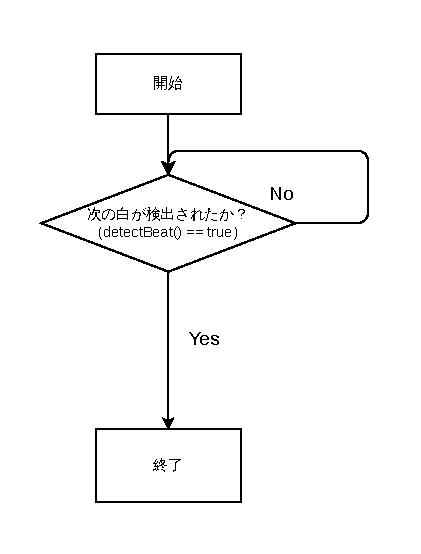
\includegraphics[width=0.8\linewidth, keepaspectratio]{figures/tantoC/onBeatDetected_drawio.pdf}
    \caption{フローチャート：onBeatDetected()}
    \label{onBeatDetected}
\end{figure}


\begin{figure}[H]
    \centering
    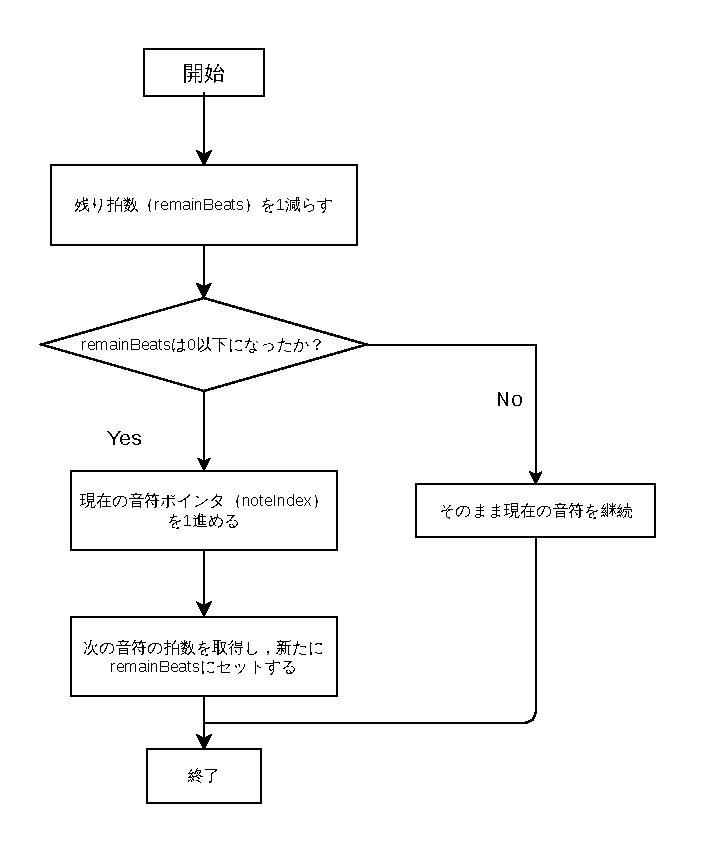
\includegraphics[width=0.6\linewidth, keepaspectratio]{figures/tantoC/advanceNote_drawio.pdf}
    \caption{フローチャート：advanceNote()}
    \label{advanceNote}
\end{figure}




\FloatBarrier



%\subsection{処理フローの設計}

%\figspace[4]{処理フロー図を挿入}

\subsection{テストの設計}
本システムの課題として，シリアル通信時の遅延と音声出力時の遅延が考えられる．そのため，結合テストとしてArduino-Processing 間の往復遅延測定を行い，遅延補正値の測定・定数化を行う．


% ===================== 担当D =====================
\section{担当D — 音響合成（Processing/Minim）}

\subsection{部品一覧}

本システムで使用する主な部品を以下に示す．
本担当は5パート分のユニットを構成するため，以下の部品を各5台用意する．

\begin{table}[h]
  \centering
  \caption{担当D 部品一覧}
  \label{tab:parts_d}
  \begin{tabular}{llrl}
    \hline
    部品名 & 型番・仕様 & 数量 & 用途 \\
    \hline
    PC（Processing実行環境） & Processing 4.x + Minim対応 & 5 & 音響合成・音声出力 \\
    スピーカーまたはヘッドフォン & — & 5 & 音声再生 \\
    USB Type-Cケーブル & — & 5 & Arduino子機との接続 \\
    \hline
  \end{tabular}
\end{table}

\subsection{ハードウェア設計}
本担当では，PC上での音響処理を主体とするため，専用の電子回路は使用しない．
Arduino子機（担当C）からUSB Type-C Serialを介してデータを受信し，
PC上のProcessing/Minimにより音響合成を行い，スピーカーへ音声出力する．

本担当は5パート分のユニットを独立して構成し，
各ユニットはArduino子機1台・PC1台・スピーカー1台の組で動作する．

なお，各PCはArduino子機1台と1対1でUSB接続されるため，
受信した4バイトパケットはそのPCが担当するパートの音響合成のみに使用する．

\begin{figure}[H]
  \centering
  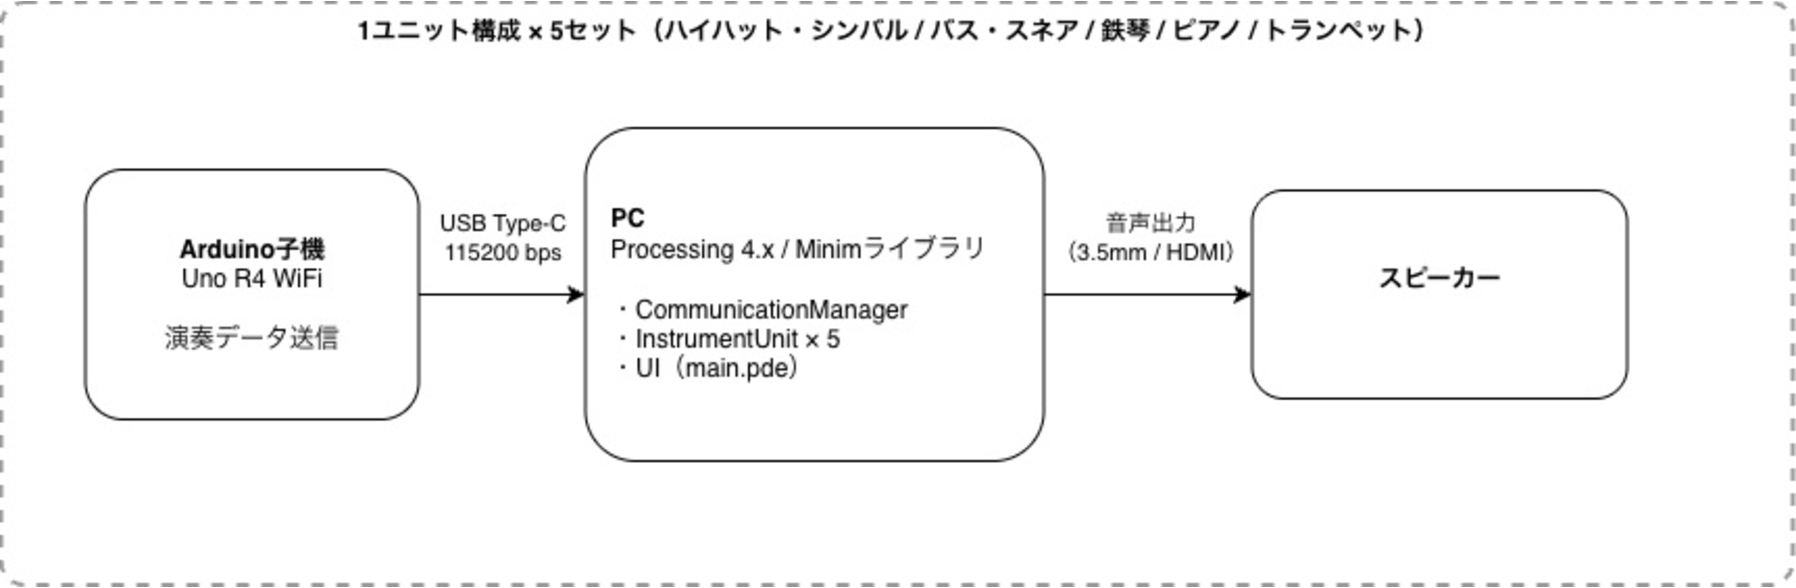
\includegraphics[width=0.85\linewidth]{figures/tantoD/hardware_connection_diagram_D.pdf}
  \caption{ハードウェア接続図（1ユニット構成 × 5セット）}
  \label{fig:hardware_D}
\end{figure}

115200\,bpsのUSBシリアル通信で4バイトパケット（NOTE\_OFF / NOTE / VEL / LONG）を受信する．

\subsection{楽器音色設計の方針}

聴衆が音楽として自然に認識できるよう，音響工学的な知見に基づき，
各ユニットに明確な役割を持たせた音色設計を行う．

\subsubsection*{楽器グループの役割}
\begin{itemize}
  \item ピアノ・鉄琴・トランペット（主旋律担当）\\
  倍音成分を調整し，メロディの明瞭さを追求する．
  基本振幅を高く設定し，常に聴衆の注意を引く音圧とする
  （基準音量1.0に対し0.8〜1.0）．

  \item バス・スネア（リズムの土台）\\
  低域のエネルギーとアタックの鋭さで拍を明示する．
  主旋律を埋もれさせない範囲で，演奏の骨格を維持するために
  十分な音圧を確保する（基準音量1.0に対し0.6〜0.7）．

  \item ハイハット・シンバル（リズムのアクセント）\\
  高域の金属音で演奏の華やかさを強調する．
  リズム楽器と同様の音量方針とする（基準音量1.0に対し0.6〜0.7）．
\end{itemize}

\subsubsection*{音色設計のアプローチ}
楽器の音色をデジタル環境で再現するにあたり，以下のプロセスに基づいた設計を行う．

\begin{enumerate}
  \item 物理特性分析：対象楽器の周波数成分を調和倍音の重なり
  （ピアノ・鉄琴・トランペット）と非調和・ノイズ成分（打楽器）に分類する．

  \item 合成手法選定：加算合成による倍音構築か，
  ホワイトノイズをベースとした減算合成か，
  目的の音響モデルに応じて決定する．

  \item 質感調整：ADSRエンベロープによる時間変化と，
  LowPass / BitCrusherによる高域・ビット深度の制御を行い，
  聴覚的な違和感を排除する．
\end{enumerate}

各パラメータの妥当性確認にあたっては，外部ツールを用いて既存音源と生成音の
スペクトラムを比較し，基音および主要倍音の構成を確認しながら
ADSRパラメータおよびフィルタ設定を逐次調整する．


\subsection{音楽的表現の設計}

指揮者のリアルタイムな動作に応じた変化が，
人間らしい演奏として知覚されるための制御方針を以下に定める．

\subsubsection*{フェルマータの自然な表現}
通信仕様をNOTE\_OFFフラグ付きパケット方式としたことで，
フェルマータの表現がより自然なものとなった．
指揮者が静止した際，担当Cが次パケットの送信を保留することで，
Processing側は特別な処理を行わずともADSRのSustain状態が自動的に延長される．
これにより，デジタル処理の不自然さを感じさせない，
生身の演奏に近い「溜め」を実現する．

演奏再開時は，腕再開後に担当Cから次パケット（NOTE\_OFF=1）が送信されることを
トリガーとしてReleaseを開始し，前の音の余韻を次音に滑らかに溶け込ませることで，
デジタル特有の不自然な音切れを回避する．

\subsubsection*{テンポ変化時の自然な追従}
テンポ変化に対し，デジタル的な違和感を排除するための配慮を組み込む．
急なテンポアップ時に前の音が残っていても，消音せずに新しい音を重ねる
多重発音を許容し，残響が途切れる不自然さを解消する（NOTE\_OFF=0時の動作）．
またテンポ加速時はRelease時間を短縮して歯切れを良くし，
減速時はReleaseを延長して空白を響きで埋めることで，
どの速度域でも自然な響きを維持する．


\subsection{楽器別音響パラメータ}

各楽器のADSR設定，倍音比率，および適用するエフェクトの数値を
表\,\ref{tab:adsr_params}に示す．
なお，表中のDecay・Release値は基準（4分音符相当）の値であり，
実装ではLONG（音価）に応じた倍率を乗じて響き・余韻の長さを調整する
（2分音符は長め，8分音符は短め）．
実装段階においては，アンサンブル全体のバランスや
指揮への追従性を考慮し，聴感上の自然さを優先して逐次微調整する方針とする．

\begin{table}[h]
  \centering
  \caption{楽器別詳細パラメータ一覧}
  \label{tab:adsr_params}
  \small
  \begin{tabular}{lp{4.5cm}cccccc}
    \hline
    楽器名 & 波形構成・倍音比率 & A {[s]} & D {[s]} & S {[lvl]} & R {[s]} & フィルタ & Bit \\
    \hline
    ピアノ
      & 9倍音（微小インハーモニシティ）＋二段減衰＋ハンマーノイズ(PINK)
      & 0.002 & 0.18／12.5 & 0 & 0.50 & 5〜10\,kHz (LP) & なし \\
    鉄琴
      & 7モード（非整数比・基音$\times$4）＋打撃ノイズ
      & 0.002 & 0.08〜1.20 & 0 & 0.85 & 14000\,Hz (LP) & 16 \\
    トランペット
      & 20倍音ウェーブテーブル＋ビブラート(5.5\,Hz)＋息ノイズ
      & 0.075 & 0.18 & 0.62 & 0.85 & 9000\,Hz (LP) & 16 \\
    バスドラム（キック）
      & body 150$\to$50\,Hz＋punch 240$\to$80\,Hz＋クリック
      & 0.001 & 0.36 & 0 & 0.10 & 4200\,Hz (LP) & 16 \\
    シンバル系
      & 非整数モード多数の加算合成（実音源STFT解析ベース）※
      & \multicolumn{6}{c}{波形生成時に内包（実効: 立上り$\approx$0.05\,s，減衰は高域ほど速く余韻長め，中心$\approx$4.8\,kHz）} \\
    \hline
  \end{tabular}
\end{table}

\noindent
※\,シンバルのみ音源を\texttt{Sampler}（事前生成したモーダル波形）とする．
波形は実音源のSTFT解析（スペクトル重心が減衰とともに約8\,kHzから約3\,kHzへ降下し，
各時刻で数百のモードをもつ特性）に基づいて生成し，アタック・減衰・スペクトル整形は
波形生成時に内包する．他楽器がOscilを音源とする点のみ異なり，
\texttt{out}への接続構造（音源UGen $\rightarrow$ 出力）は全楽器で共通である．

\vspace{0.3em}
\noindent
注\,A/D/S/R欄は主要成分の代表値である．ピアノ・鉄琴は倍音（モード）ごとに個別のADSRをもち，
ピアノは二段減衰（プロンプト約0.18\,s＋アフターサウンド約12.5\,s）でBitCrusherは不使用．
バスドラムはドラムセットのキックを対象とし，振幅・ピッチを\texttt{Line}で整形する．

\subsection{ソフトウェア設計}

\subsubsection{ファイル構成}

本システムはProcessingスケッチとして実装し，以下の構成とする．

\begin{itemize}

  \item \texttt{main.pde} \\
  システム全体の制御を行う．
  初期化（\texttt{setup()}），メインループ（\texttt{draw()}），
  およびUIコンポーネント（ポート自動接続・マスターボリューム・受信データモニタ）を含む．

  \item \texttt{CommunicationManager.pde} \\
  シリアル通信の受信および4バイトデータのパース処理を行う．
  NOTE\_OFFフラグに基づく前音消音および新規発音イベントを生成し，InstrumentUnitへ通知する．
  各PCは担当パートのInstrumentUnit1インスタンスのみに通知する．

  \item 楽器別ファイル（\texttt{piano.pde}, \texttt{tekkinn.pde}, \texttt{toranpet.pde}, \texttt{basudoramu.pde}, \texttt{sinbaru.pde}）\\
  各ファイルは\texttt{InstrumentUnit}クラスを定義し，担当楽器の音響生成処理・音色管理を行う．
  各PCは担当楽器のスケッチのみを実行する．
  UGenチェーンの構築，音高変換，発音・消音制御を統括する．
  多重発音に対応するため，発音ごとにボイス（楽器インスタンス）を生成し，
  リスト（\texttt{activeVoices}）で管理する動的な多重発音構成とする．

\end{itemize}


\subsubsection{オブジェクト設計（クラス図）}

\begin{figure}[H]
  \centering
  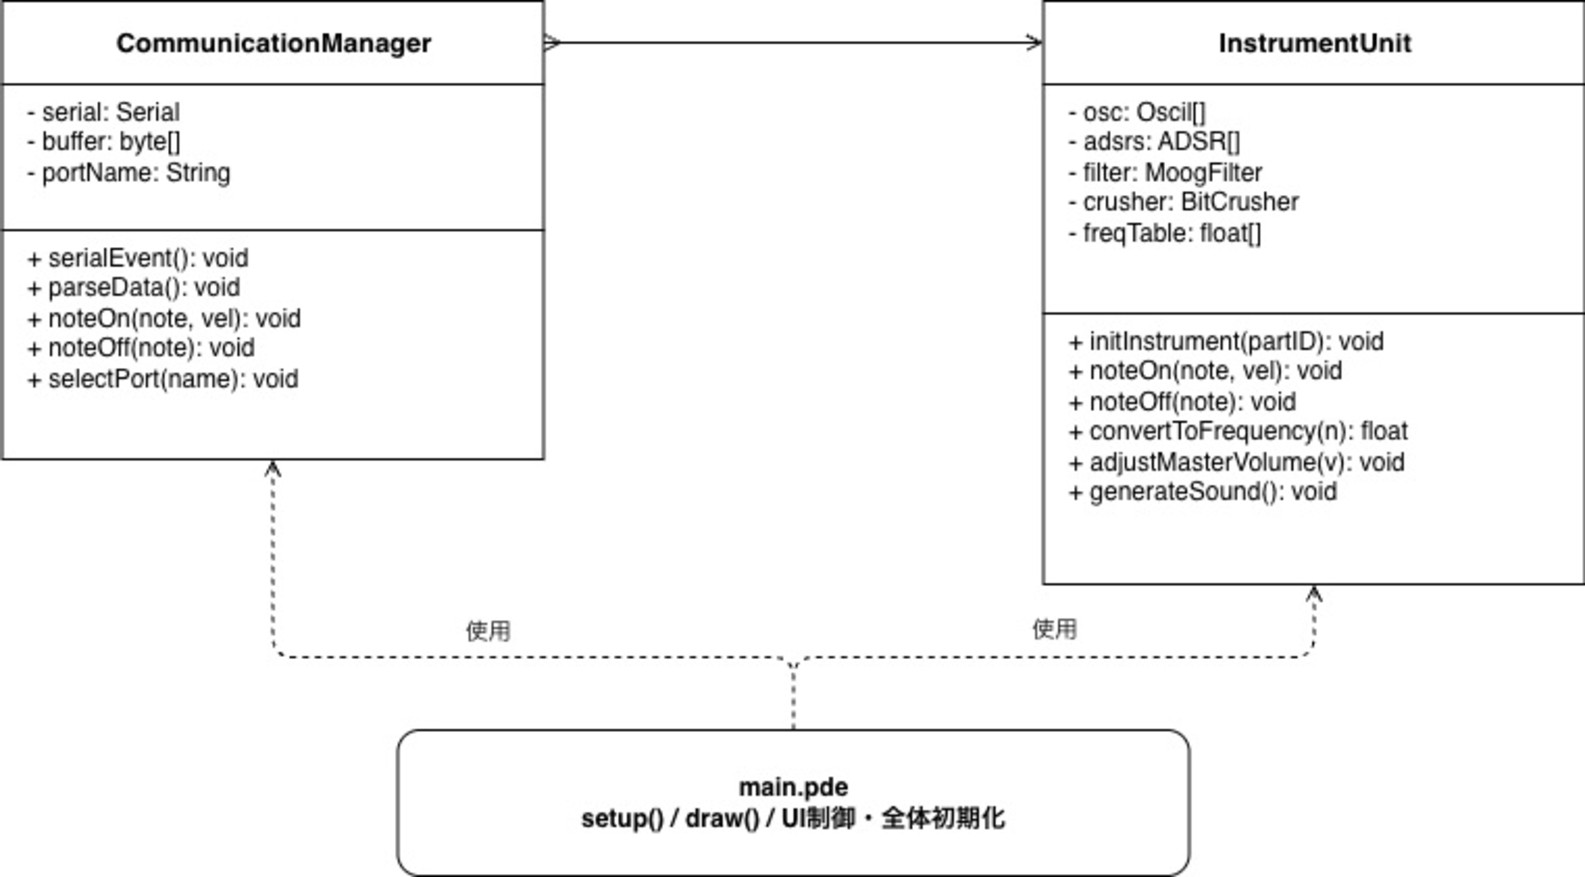
\includegraphics[width=0.85\linewidth]{figures/tantoD/class_diagram_D.pdf}
  \caption{クラス図（CommunicationManager / InstrumentUnit / main.pde）}
  \label{fig:class_D}
\end{figure}

本システムは以下の主要クラスで構成される．

\begin{itemize}

  \item \texttt{CommunicationManager} \\
  シリアル通信の受信および4バイトパケット（NOTE\_OFF / NOTE / VEL / LONG）の
  パースを行い，前音消音および新規発音イベントをInstrumentUnitへ通知する．
  パート種別は各PCのシリアル接続で確定するため，NOTEバイトはすべて
  音名インデックス（0〜5または6）として解釈する．

  \item \texttt{InstrumentUnit} \\
  受信イベントに基づき，音高変換，楽器選択，
  およびUGenチェーンによる音響生成処理を統括する．
  発音ごとにボイス（楽器インスタンス）を生成してリスト（\texttt{activeVoices}）で管理し，
  NOTE\_OFFフラグ=0の場合は前音を残したまま新規ボイスを重ね，
  NOTE\_OFFフラグ=1の場合はボイスをReleaseへ移行させてリストから除去することで
  多重発音を実現する．

\end{itemize}

音名インデックスからの周波数変換は，
平均律式 $f = 440 \times 2^{(n-69)/12}$\,[Hz] を用いる．
インデックスとMIDIノート番号の対応を表\,\ref{tab:midi_table}に示す．

\begin{table}[H]
  \centering
  \caption{音名インデックス → MIDIノート番号 → 周波数 変換テーブル}
  \label{tab:midi_table}
  \begin{tabular}{cccc}
    \hline
    インデックス（担当C） & 音名 & MIDIノート番号 $n$ & 周波数 $f$\,[Hz] \\
    \hline
    0   & C4（ド） & 60              & 261.63 \\
    1   & D4（レ） & 62              & 293.66 \\
    2   & E4（ミ） & 64              & 329.63 \\
    3   & F4（ファ）& 65             & 349.23 \\
    4   & G4（ソ） & 67              & 392.00 \\
    5   & A4（ラ） & 69（基準）      & 440.00（基準） \\
    \hline
    6   & 休符     & —               & 発音なし \\
    \hline
  \end{tabular}
\end{table}

Velocityは0〜127の値をADSRのSustainレベル（0.0〜1.0）へ正規化し，
音量制御に反映する．
LONGバイトは音価（\texttt{2}=2分音符 / \texttt{4}=4分音符 / \texttt{8}=8分音符）を示し，
新規発音時にADSRの減衰（Decay）およびリリース（Release）時間へ倍率として反映することで，
響き・余韻の長さを調整する（2分音符は長め，4分音符は標準，8分音符は短め）．
発音中の音を実際に停止するタイミングはLONGではなくNOTE\_OFF=1の受信で制御する．

NOTE\_OFFフラグ=1のパケット受信時には前音ボイスの\texttt{noteOff()}を呼び出し，
続くNOTEバイトが休符（6）でなければ新規ボイスを生成して\texttt{noteOn()}で発音を開始する．
フェルマータ中は担当Cが次パケットの送信を保留するため，
Sustainが自動的に延長される．
NOTE\_OFFフラグ=0の場合は前音を消音せずに新規発音を重ねることで多重発音を実現する．

\subsubsection{関数設計}

主要な関数を以下に示す．

\begin{itemize}

  \item \texttt{setup()} \\
  Minim，AudioOutput，およびシリアル通信の初期化を行う．
  各楽器パートのInstrumentUnitインスタンスを生成し，
  UGenチェーンをAudioOutputへ接続する．

  \item \texttt{draw()} \\
  メインループとして動作し，
  UIコンポーネント（受信データモニタ・マスターボリューム）の描画更新を行う．

  \item \texttt{serialEvent()} \\
  シリアルデータ受信時に自動的に呼び出され，
  受信バイトをバッファへ格納する．

  \item \texttt{parseData()} \\
  受信バッファから4バイト単位でデータを取り出し，
  NOTE\_OFF（\texttt{1}=前音停止 / \texttt{0}=継続），
  音名インデックス，Velocity，LONG（音価）を抽出して
  前音消音および新規発音イベントに変換する．
  NOTEバイトはすべて音名インデックス（0〜5または6）として解釈し，
  パートIDの抽出は行わない．

  \item \texttt{noteOn(int noteIndex, int velocity, int noteLength)} \\
  音名インデックスを周波数に変換し，
  新規ボイス（楽器インスタンス）を生成して\texttt{activeVoices}へ追加し，
  そのボイスの\texttt{noteOn()}でアタックを開始する．
  Velocityを正規化して振幅に反映し，
  noteLength（音価）に応じてADSRの減衰・リリース時間に倍率を乗じ，響きの長さを調整する．
  なお消音は本関数では行わず，NOTE\_OFF=1受信時の\texttt{noteOff()}で制御する．

  \item \texttt{noteOff(int noteIndex)} \\
  該当する音名インデックスのボイスを\texttt{activeVoices}から検索し，
  \texttt{noteOff()}でReleaseへ移行させたうえでリストから除去する．

  \item \texttt{convertToFrequency(int noteIndex)} \\
  音名インデックスをMIDIノート番号へ変換し，
  $f = 440 \times 2^{(n-69)/12}$\,[Hz] により周波数を算出する．

  \item \texttt{InstrumentUnit(AudioOutput out)}（コンストラクタ） \\
  各PCは担当楽器専用のスケッチを実行するため，パートIDによる選択は行わない．
  コンストラクタで当該楽器のUGenチェーン（Oscil・ADSR・Filter・BitCrusher）を構築し，\texttt{out}へ接続する．
  楽器ごとのADSRパラメータおよびフィルタ設定を適用する．
  ただしシンバルのみ，音源をOscilではなく\texttt{Sampler}（事前生成したモーダル波形）とし，
  同様に\texttt{out}へ接続する（接続構造は他楽器と共通）．

  \item \texttt{adjustMasterVolume(float value)} \\
  UIスライダーからの入力（0.0〜1.0）をデシベルに変換し，
  \texttt{out.setGain()}を呼び出して出力音量を調整する．

\end{itemize}

\subsection{処理フローの設計}

本システムの処理は，初期化フローと実行時フローの2つに分けて設計する．

\begin{figure}[H]
  \centering
  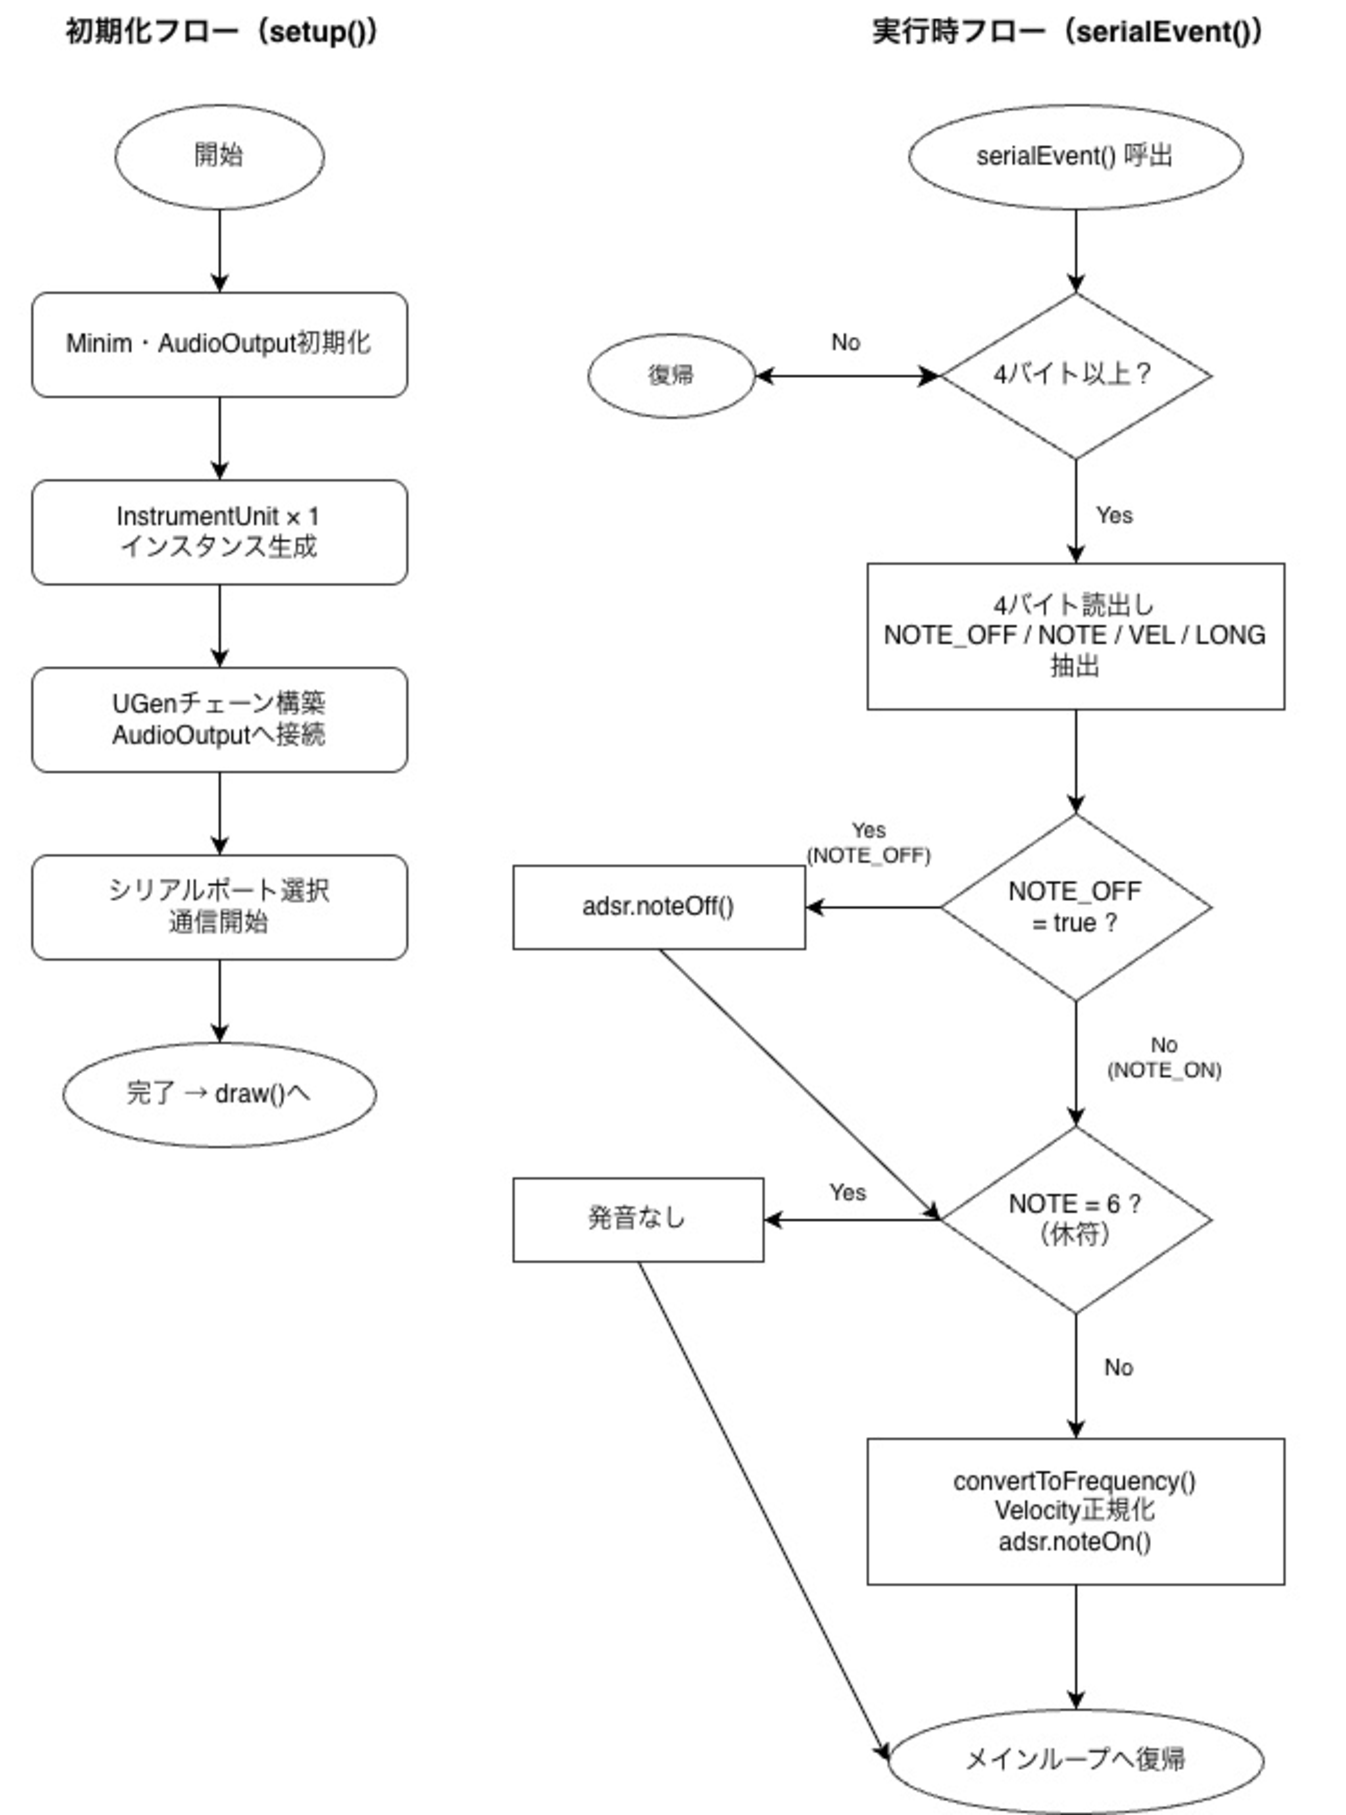
\includegraphics[width=0.85\linewidth]{figures/tantoD/process_flow_diagram_D.pdf}
  \caption{処理フロー図（初期化フロー・実行時フロー）}
  \label{fig:process_flow_D}
\end{figure}

\subsubsection*{初期化フロー（\texttt{setup()}）}

\begin{enumerate}
  \item Minimおよびシリアル通信を初期化する
  \item 担当パートに対応するInstrumentUnit（1インスタンス）を生成する
  \item UGenチェーンを構築し，AudioOutputへ接続する
  \item シリアルポートへ自動接続し，通信を開始する
\end{enumerate}

\subsubsection*{実行時フロー（\texttt{serialEvent()} → \texttt{parseData()}）}

\begin{enumerate}
  \item シリアルバッファに4バイト以上蓄積されているか確認する
  \item 4バイトを読み出し，NOTE\_OFF・音名インデックス・Velocity・LONGを抽出する
  \item NOTE\_OFFフラグを判定する
  \begin{itemize}
    \item NOTE\_OFF = \texttt{1}（前音停止）の場合：
    \begin{enumerate}
      \item 現在発音中のボイスを\texttt{noteOff()}し，
            Releaseフェーズへ移行させてリストから除去する
    \end{enumerate}
    \item NOTE\_OFF = \texttt{0}（継続）の場合：
    \begin{enumerate}
      \item 前音の消音は行わない（多重発音）
    \end{enumerate}
  \end{itemize}
  \item 音名インデックスが6（休符）であれば新規発音せずに終了する
  \item \texttt{convertToFrequency()}で周波数を算出する
  \item Velocityを正規化して振幅に反映する
  \item LONG（音価）に応じてADSRの減衰・リリース時間に倍率を乗じ，響きの長さを設定する
  \item 新規ボイスを生成して\texttt{activeVoices}へ追加し，\texttt{noteOn()}でアタックを開始する
  \item メインループへ復帰する
\end{enumerate}

フェルマータ中は担当Cが次パケットの送信を保留するため，
Processing側は追加処理なくSustain状態が自動的に延長される．
腕再開後に次パケット（NOTE\_OFF=1）を受信した時点でReleaseへ移行し，
続く音名インデックスに基づき次音の発音を開始する．


\subsection{MOE / MOP / TPM}

\subsubsection*{MOE — 有効指標}

\begin{table}[H]
  \centering
  \caption{担当D MOE一覧}
  \label{tab:moe_d}
  \begin{tabular}{llp{8cm}}
    \hline
    ID & 指標 & 説明 \\
    \hline
    MOE-D1 & 音楽的に正確な発音・消音
           & 受信したNOTE情報を正しい音高・音色・タイミングで
             発音・消音できる \\
    MOE-D2 & 楽器らしい音色の実現
           & 各楽器（ハイハット・バス・鉄琴・ピアノ・トランペット）が
             聴衆に識別できる音色を持つ \\
    \hline
  \end{tabular}
\end{table}

\subsubsection*{MOP — 性能指標}

\begin{table}[H]
  \centering
  \caption{担当D MOP一覧}
  \label{tab:mop_d}
  \begin{tabular}{llp{3.5cm}p{5cm}}
    \hline
    ID & 性能指標 & 目標値 & 測定方法 \\
    \hline
    MOP-D1 & 受信→発音遅延
           & $\leq 50$\,ms
           & C2テスト: パケット受信タイムスタンプとMinimの
             発音開始を計測（可能であればオシロ） \\
    MOP-D2 & 消音確実性
           & NOTE\_OFF=1受信後 $\leq 100$\,ms以内に確実に消音
           & C2テスト: 録音データで消音タイミングを確認 \\
    MOP-D3 & 音高精度
           & 指定音名との誤差 $\pm 5$\,cent以内
           & チューナーアプリで各音名の発音周波数を計測 \\
    MOP-D4 & Serial受信エラーなし
           & 通し演奏中に受信パースエラー 0回
           & S1テスト: エラーカウンタ変数をシリアルで監視 \\
    \hline
  \end{tabular}
\end{table}

\subsubsection*{TPM — 技術性能指標（開発中に継続監視）}

\begin{table}[H]
  \centering
  \caption{担当D TPM一覧}
  \label{tab:tpm_d}
  \begin{tabular}{lp{4cm}p{3cm}p{4.5cm}}
    \hline
    ID & 監視項目 & 監視タイミング & 判定基準 \\
    \hline
    TPM-D1 & 4バイト受信パーサの動作確認
           & 修正後・P7テスト時
           & \texttt{NOTE\_OFF=1}で前音消音，
             \texttt{0}で継続が
             正しくトリガーされること \\
    TPM-D2 & 音名インデックス→周波数変換の整合性
           & 実装着手時（C-D合意後）
           & C4=0のインデックスが
             $f=261.6$\,Hzに変換されること \\
    TPM-D3 & ADSRパラメータの音色調整状況
           & 実装中・P7テスト時
           & 各楽器が識別可能な音色を持ち，
             音量バランスが取れていること \\
    TPM-D4 & Minimライブラリ動作環境の統一
           & 実装着手前
           & 5台のPC全てでProcessing + Minimが
             正常動作すること（バージョン統一） \\
    TPM-D5 & \texttt{out.setGain()}の動作確認
           & P7テスト時
           & スライダー操作により音量が0〜100\,\%の
             範囲で連続的に変化すること \\
    \hline
  \end{tabular}
\end{table}

\subsection{テストの設計}

本システムのテストは，事前確認テスト・結合テスト・システムテストの
3フェーズで実施する．
なお，P7が事前確認テスト，C2が結合テスト，S1がシステムテストにそれぞれ対応する．
各テストの内容および合格基準を表\,\ref{tab:test_d}に示す．

\begin{table}[H]
  \centering
  \caption{担当D テスト計画}
  \label{tab:test_d}
  \begin{tabular}{llp{5cm}p{4cm}}
    \hline
    ID & テスト名 & 内容 & 合格基準 \\
    \hline
    P7 & Processing音響出力確認
       & 手動で4バイト（NOTE\_OFF=1, NOTE, VEL, LONG）を
         シリアル送信し，指定音が発音されるか確認する
       & 正しい音高・音量で発音される \\
    C2 & C-D間同期確認
       & Arduinoのパケット送信から発音までの遅延を計測する．
         またNOTE\_OFF=1受信時に確実に前音が消音されるか確認する
       & 遅延 $\leq$ 50\,ms，NOTE\_OFF=1時に確実に消音，
         発音ずれ $\leq$ 1拍 \\
    S1 & 通し演奏・BPM維持評価
       & 全15小節以上の通し演奏で音響品質・タイミングを評価する
       & BPM誤差 $\pm$5\,bpm以内，発音ミスなし \\
    \hline
  \end{tabular}
\end{table}

また，開発中の音色調整を目的として，以下の評価を随時実施する．

\begin{itemize}
  \item 音高精度確認 \\
  チューナーアプリで各音名の発音周波数を計測し，
  目標値との誤差が$\pm$5\,cent以内であることを確認する．

  \item 聴感評価 \\
  各楽器音が聴衆に識別可能な音色を持つことを
  人間の聴感により確認する．
\end{itemize}

% =============================================================
\chapter{変更履歴}\label{chap:revision-history}

本章では，前回提出から今回提出までに行った
マネジメント計画書および基本設計書・詳細設計書に対する修正履歴を記録する．

% 直近の変更履歴（課題1・課題2 用）
% management_plan.tex の \chapter{変更履歴} から \input される．
%
% ライフサイクル:
%   - 変更があったら，このファイルに行を追記する（書式は下記）
%   - 提出のタイミングで，下記の履歴行を revision_history/sections/changelog.tex
%     （累積版・課題3用）の末尾にコピーしてから，このファイルの履歴行を全て削除する
%
% 書式:
%   YYYY-MM-DD & 学籍番号 : 氏名 & 対象（章・節） & 変更内容 \\
%
% 前提パッケージ（呼び出し側でロード済みであること）:
%   \usepackage{longtable}
%   \usepackage{booktabs}
%   \usepackage{array}

\begin{longtable}{p{2.2cm}p{3.5cm}p{4cm}p{5.5cm}}
\toprule
日付 & 担当 & 対象（章・節） & 変更内容 \\
\midrule
\endfirsthead

\toprule
日付 & 担当 & 対象（章・節） & 変更内容 \\
\midrule
\endhead

% --- 履歴行をここに追記していく（提出時にクリア） ---
2026-07-01 & 24G1056 : 慶田 優 & 第6章 テスト実施記録 & INT-5（カラーセンサ＋フォトトランジスタ統合テスト）の結果を追記（不合格：環境光によるS13683認識不安定） \\
2026-07-01 & 24G1056 : 慶田 優 & 第5章 TPM測定推移 & TPM-2（拍検出成功率）を3時点分追記（6/17単体≈100\%○，6/24結合≈90\%×，7/1測定不能×）．TPM-4（EMA収束拍数：約1拍○）・TPM-5（最大追従BPM：110bpm○）を追記 \\
2026-07-01 & 24G1056 : 慶田 優 & 第4章 TRL評価 & 拍タイミング検出の根拠にS13683環境光問題を追記．テンポ推定の根拠を「3拍以内」から「約1拍以内（TPM-4実測値）」に更新．テンポ追従演奏（TRL1→3），カラーLED制御（輝度エンコードLEDから改称・根拠更新），演奏状態遷移管理（TRL2→3）を更新 \\

\bottomrule
\endfoot
\end{longtable}


% =============================================================
% 参考文献
\begin{thebibliography}{9}

\bibitem{sudo2007}
  須藤宏明，他，
  「複数演奏者による音楽リズムタイミングの一致度の測定と脳波への影響の考察」，
  \textit{日本感性工学会研究論文集}，Vol.7，No.2，pp.337--344，2007年．

\bibitem{kawase}
  河瀬諭，
  「合奏における演奏者間コミュニケーション――タイミング調整とその手がかり――」，
  \textit{心理学研究}，Vol.57，No.4，pp.495--，日本心理学会．

\bibitem{jnd1974}
  「短音の提示間隔と周波数および音圧のJND」，
  \textit{Audiology Japan}，Vol.17，No.5，pp.399--400，1974年．

\end{thebibliography}

\end{document}
